% REMEMBER: You must not plagiarise anything in your report. Be extremely careful.

\documentclass{l4proj}

    
%
% put any additional packages here
%

\begin{document}

%==============================================================================
%% METADATA
\title{Level 4 Project Report Template}
\author{John H. Williamson}
\date{September 14, 2018}

\maketitle

%==============================================================================
%% ABSTRACT
\begin{abstract}
    Every abstract follows a similar pattern. Motivate; set aims; describe work; explain results.
    \vskip 0.5em
    ``XYZ is bad. This project investigated ABC to determine if it was better. 
    ABC used XXX and YYY to implement ZZZ. This is particularly interesting as XXX and YYY have
    never been used together. It was found that  
    ABC was 20\% better than XYZ, though it caused rabies in half of subjects.''
\end{abstract}

%==============================================================================

% EDUCATION REUSE CONSENT FORM
% If you consent to your project being shown to future students for educational purposes
% then insert your name and the date below to  sign the education use form that appears in the front of the document. 
% You must explicitly give consent if you wish to do so.
% If you sign, your project may be included in the Hall of Fame if it scores particularly highly.
%
% Please note that you are under no obligation to sign 
% this declaration, but doing so would help future students.
%
%\def\consentname {My Name} % your full name
%\def\consentdate {20 March 2018} % the date you agree
%
\educationalconsent


%==============================================================================
\tableofcontents

%==============================================================================
%% Notes on formatting
%==============================================================================
% The first page, abstract and table of contents are numbered using Roman numerals and are not
% included in the page count. 
%
% From now on pages are numbered
% using Arabic numerals. Therefore, immediately after the first call to \chapter we need the call
% \pagenumbering{arabic} and this should be called once only in the document. 
%
% Do not alter the bibliography style.
%
% The first Chapter should then be on page 1. You are allowed 40 pages for a 40 credit project and 30 pages for a 
% 20 credit report. This includes everything numbered in Arabic numerals (excluding front matter) up
% to but excluding the appendices and bibliography.
%
% You must not alter text size (it is currently 10pt) or alter margins or spacing.
%
%
%==================================================================================================================================
%
% IMPORTANT
% The chapter headings here are **suggestions**. You don't have to follow this model if
% it doesn't fit your project. Every project should have an introduction and conclusion,
% however. 
%
%==================================================================================================================================
\chapter{Introduction}

% reset page numbering. Don't remove this!
\pagenumbering{arabic} 


\section{Concurrency and Distributed Systems}
Concurrency and distributed systems are becoming increasingly important in modern computational science, especially in the context of cloud computing and big data. \cite{sutter_2005_software} emphasize that with the proliferation of multicore processors, the software industry needs to adopt new tools and ways of thinking in order to fully utilize the potential of multicore processors. Concurrency refers to the ability of a system to handle multiple tasks at the same time, which allows efficient use of computational resources. For example, by processing hundreds or even thousands of client requests in parallel, modern Web servers are able to dramatically improve response times and system throughput. This shift in demand requires mainstream software development to stop ignoring concurrency, a challenge that requires developers to master the design and implementation of concurrent programs (\cite{sutter_2005_software}).
    
The design of Multiplayer Online Role-Playing Game (MMORPG) servers, such as exemplified by the \cite{glenday_guinness} (Figure \ref{fig:WoWlogo}) demonstrates the value of concurrent programming in real-world applications, where the use of a client-server model and event-driven architecture enables asynchronous processing of player requests. \cite{kim_2018_design} study, by utilizing Input/Output Completion Port (IOCP) and multithreading techniques, has demonstrated methods to effectively improve server performance, handle concurrent connections and employ fine-grained locking mechanisms for access control of shared resources to reduce the risk of deadlock and effectively improve system responsiveness and throughput.

\begin{figure}[h]
    \centering
    \begin{minipage}[t]{0.35\textwidth}
        \centering
        
\includegraphics[width=\linewidth,height=5cm,keepaspectratio]{images/WoWlogo.png}
        \caption{World of Warcraft}
        \label{fig:WoWlogo}
    \end{minipage}
    \quad
    \begin{minipage}[t]{0.30\textwidth}
        \centering
        \includegraphics[width=\linewidth,height=5cm,keepaspectratio]{images/PokemonGo.jpeg}
        \caption{Pokemon GO}
        \label{fig:PokemonGo}
    \end{minipage}
\end{figure}

On the other hand, Distributed systems achieve workload decentralization by assigning tasks across multiple compute nodes, which is especially critical for processing large-scale data sets. For example, the distributed architecture of \cite{wikipediacontributors_2019_pokmon} demonstrates the efficient ability of distributed systems to manage and synchronize millions of players globally, through a network of servers deployed in multiple locations around the world, and the use of geo-distributed database technology to decentralize the storage of data based on the geographic location of players, showing the importance of this technology in dealing with large-scale, real-time interactive applications.
		
The combination of concurrency and distributed systems not only greatly improves the efficiency of task processing, but also enhances the reliability and scalability of the system. In the case of distributed databases, for example, data is replicated across multiple nodes, ensuring that the entire system can maintain normal operation even if some of the nodes fail. In addition, this technology supports the dynamic adjustment of computing resources according to actual demand, a feature that is widely used in cloud service platforms such as \cite{aws_2023_amazon} and \cite{microsoft_2023_cloud}. This exposition not only demonstrates the key role of concurrent programming in ensuring high availability and optimizing user experience, but also provides an important reference for designing efficient concurrent and distributed systems.

\section{Challenges}

While these systems are capable of handling unprecedented amounts of data and computational tasks, they also introduce a new set of challenges. 

\subsection{Thread Deadlock}

Thread deadlocks are a common problem in concurrent programming, which in short means that no thread is able to continue execution due to circular locking or communication dependencies. For example, if two threads each occupy a portion of a resource and are waiting for the other to release its resource in order to continue execution, this creates a deadlock. This situation is particularly common in database transactions and operating system resource allocation, and it can seriously affect the stability and efficiency of a program.

\subsection{Communication Mismatch}

Communication mismatch is another critical issue in distributed systems. Nodes in a distributed environment need to exchange information frequently, and any inconsistency in communication protocols or data formats can lead to major failures. Taking microservice architecture as an example, if the communication interfaces between services are not clearly defined or fail to maintain compatibility during version updates, it may lead to the functional failure of the whole system. This is particularly noticeable in fast iterative and multi-team projects and requires special attention.

\section{Case Study: The Mailbox Mechanism}

When exploring the field of concurrent programming in depth, actor modeling languages, such as Erlang, provide an effective concurrent programming paradigm. By introducing mailboxes as a communication mechanism, these languages allow processes to collaborate with each other in a message-passing fashion, effectively avoiding the locking and shared state management problems of traditional concurrent programming. However, while mailboxes serve as a bridge between actors, they do not explicitly constrain the types of messages and can only process messages in the order they are received, which is not sufficient to deal with an inherently unorganized message flow.

Building on this, the Pat language, an emerging language in the research field, introduces the notion of mailboxes and mailbox types for first-class. Compared with traditional actor modeling languages, the Pat language is designed to emphasize the importance of mailbox types, and further enhance the security and maintainability of concurrent programs by constraining the types and processing order of messages in the mailboxes through a type system.This innovative point of the Pat language not only simplifies the complexity of concurrent programming, but also provides new perspectives and tools for research in the field of concurrent and distributed programming.

In further exploring the application of the Pat language in the field of concurrent programming, this paper aims to show how mailbox types in the Pat language can effectively manage concurrent tasks by introducing a concrete code example. As we see in Listing \ref{lst:patexample1}, By defining the \textbf{Tasks interface} and its implementation, the message type in the mailbox is forced to be constrained to String. The sample code clearly shows the process of producing and consuming tasks, where the \textcolor{blue}{produceTasks} function is responsible for sending tasks to instances of the Tasks interface, and the \textcolor{blue}{consumeTasks} function is responsible for receiving and executing these tasks.The Pat language utilizes the concurrency primitive \textbf{spawn} to implement the parallel execution of functions. Thus, tasks are produced and consumed simultaneously in different execution streams. 

\noindent\begin{minipage}{\linewidth}
\lstset{style=patstyle}
\begin{lstlisting}[caption=Pat Language Example, label={lst:patexample1}]
interface Tasks {
  Task(String)
}

def produceTasks(mb : Tasks!) : Unit {
  mb ! Task("task1");
  mb ! Task("task2")
}

def consumeTasks(self: Tasks?) : Unit {
  guard self: Task {
    free -> ()
    receive Task(i) from self ->
        print(i);
        consumeTasks(self)
  }
}

def main(): Unit {
  let task = new[Tasks] in
  spawn { produceTasks(task) };
  consumeTasks(task)
}

main()
\end{lstlisting}
\end{minipage}

\section{Research Goals}

The aim of this research is to develop a runtime interpreter specifically designed to support a new programming language, the Pat language.The Pat language addresses the programming challenges of concurrency and distributed systems, and by introducing advanced concurrent programming primitives and a unique mailbox type system, it aims to provide developers with a more intuitive and concise way to handle concurrent tasks and communication flows. While a type checker for the Pat language has been implemented, an efficient execution environment has yet to be developed. The main goal of this project is to build such an execution environment so that developers can easily write, test and run programmes written in the Pat language.

This interpreter should not only satisfy the runtime requirements of a general programming language, such as memory management, but should also focus on the specific needs of concurrent and distributed computing. By providing such a tool, the Pat language will become a powerful support for the research and development of concurrent and distributed systems, which not only promotes the wide application and continuous development of the Pat language, but also provides new perspectives and methods for exploring problems in the field of concurrent programming, and establishes a solid foundation for future technological innovations.

\section{Outline}
This dissertation organized into the following structure:

\begin{itemize}
  \item \textbf{Chapter 2} introduces the need for concurrent programming, and discusses the definition, differences, and relative advantages and disadvantages of channels and actors. It also examines the mailbox type system, its significance in concurrent programming, and outlines scheduling algorithms and their implementation in OCaml.
  
  \item \textbf{Chapter 3} identifies the essential functionalities required for the project, desirable features, and potential enhancements. It delineates the scope of the current phase by highlighting the aspects of research that are not addressed.
  
  \item \textbf{Chapter 4} details the application of the CEK mechanism within the Pat language. It elucidates the rationale behind choosing CEK over CPS and describes the design of Pat's scheduling and garbage collection mechanisms.
  
  \item \textbf{Chapter 5} covers the implementation of the CEK machine, the communication and scheduling mechanisms within Pat's mailbox system, the current state of garbage collection, and the development of both the evaluation step printer and the error-handling mechanism.
  
  \item \textbf{Chapter 6} assesses the system's performance using correctness and runtime tests, includes a critical evaluation, and discusses the outcomes and potential areas for improvement.
  
  \item \textbf{Chapter 7} reviews Pat language's principal contributions, summarizes the findings of the thesis, and proposes future work directions and potential research application areas.
\end{itemize}


%==================================================================================================================================
\chapter{Background}

\section{Concurrency}
Modern concurrent programming uses two main paradigms: Message-Passing Concurrency and Shared-Memory Concurrency, which use different strategies and mechanisms to handle concurrent tasks.

\subsection{Shared Memory}
Shared-memory concurrency model allows multiple processes or threads to share the same memory space and communicate through this shared space. While this approach improves efficiency in certain scenarios, it also introduces data consistency and synchronisation issues. In the shared memory model, developers must carefully handle locking mechanisms and synchronisation issues to prevent deadlocks and race conditions from occurring.Java and C++ are examples of languages that support this concurrency model.

Here is a quick Java example(Listing \ref{lst:deadlockExample}), if \textcolor{red}{Thread1} successfully acquires \textbf{lock1} and \textcolor{red}{Thread2} acquires \textbf{lock2} at the same time, and then each of them tries to acquire a lock already held by the other, this leads to a classic deadlock situation. Both threads will wait indefinitely because the locks they each hold will not be released:

\lstset{style=javastyle}
\begin{lstlisting}[caption={Java example demonstrating a potential deadlock}, label={lst:deadlockExample}]
......

new Thread(() -> {
    synchronized (lock1) {
        System.out.println("Thread 1: Holding lock 1...");
        try { Thread.sleep(100); } catch (InterruptedException e) {}
        System.out.println("Thread 1: Waiting for lock 2...");
        synchronized (lock2) {
            System.out.println("Thread 1: Holding lock 1 and 2...");
        }
    }
}).start();
        
new Thread(() -> {
    synchronized (lock2) {
        System.out.println("Thread 2: Holding lock 2...");
        try { Thread.sleep(100); } catch (InterruptedException e) {}
        System.out.println("Thread 2: Waiting for lock 1...");
        synchronized (lock1) {
            System.out.println("Thread 2: Holding lock 1 and 2...");
        }
    }
}).start();

......
\end{lstlisting}

\subsection{Message Passing}
In contrast, Message-passing Concurrency is a programming paradigm that enables communication and coordination by sending and receiving messages between processes or threads. The main advantage of this approach is that it provides a clear mechanism to avoid data contention and conflict, as data is passed through message exchange rather than sharing. In this model, each process or thread has a separate memory space and all communication takes place through well-defined message interfaces, but additional overhead is introduced(\cite{a2023_message}).The Erlang language and the Akka framework are excellent representatives of this model.

Although message-passing concurrency and shared-memory concurrency each have their own strengths, message-passing concurrency provides a clearer and more controlled approach to dealing with the problems of distributed systems and reducing complex synchronisation issues. Therefore, the message-passing concurrency paradigm was chosen in the design of the Pat language in order to provide a safer and more intuitive approach to concurrent programming.

\section{Communication Mechanisms}
With its clear communication mechanism, the message-passing concurrency model provides the Pat language with an effective means to avoid data conflicts and competition, which significantly enhances the advantages of concurrent program design. On this basis, by introducing two high-level abstractions, Channel and Actors, not only the expressive ability of message-passing concurrency is further enhanced, but also the manageability and extensibility of concurrent programs are significantly improved (Figure \ref{fig:channel_actor}). Nevertheless, both models have revealed some problems in practice.

\subsection{Channel}
The channel model, especially widely used in languages such as Go, facilitates message passing between processes or threads by naming channels. As shown in the Figure \ref{fig:channel_actor}.a, processes or threads communicate and coordinate with each other by passing messages through these channels. These named channels allow messages to be exchanged between different execution units and are a key mechanism in concurrent programming. However, the use of channels is not without challenges, especially when it comes to synchronization issues. These problems stem mainly from communication mismatches and channel-based deadlocks, for example, when two processes are both waiting to receive data on the same channel, or when they try to send data on a channel blocked by a receive operation. These types of deadlocks and communication mismatches are common challenges in concurrent programming in the channel model.

Implementing channels in a distributed environment is more complex, as discussed by \cite{chaudhuri_2009_a} in his paper "Concurrent ML Library in Concurrent Haskell", which is mainly attributed to the complexity of the distributed abstract state machine required for synchronization. Channels, points, and synchronizers interact according to rules and states defined for each entity to facilitate operations and transitions. In turn, state changes of entities lead to the complexity of implementing channels. In addition, the implementation of channels in a distributed environment involves not only communication structures and types, but also how to handle complex interaction patterns such as iteration, branching, and delegation(\cite{hu_sessionbased}). These researches show that while channel messaging between processes or threads explicitly specifies the type of data transferred by the channel, ensuring deadlock-free and efficient communication in distributed systems is a challenge.


\subsection{Actor}
In contrast, the actor model, first proposed by \cite{hewitt_a} and implemented in languages such as Erlang, demonstrates the efficiency and generalizability of the actor model for AI languages dealing with the need for high parallelism. The model focuses on enabling each individual actor entity to interact via asynchronous message passing. According to Figure \ref{fig:channel_actor}.b, where each Actor is an addressable process with a message queue or mailbox for receiving messages. Each Actor is a separate entity that interacts via asynchronous message passing. This model is particularly well suited for building large-scale, scalable distributed applications, providing natural support for distributed computing, especially in terms of fault tolerance and system reliability. \cite{agha_1985_actors} points out that the Actor model has addressed key challenges in distributed computing, such as deadlocks and divergence. However, the actor model faces challenges in implementing type safety, and in the case of Akka, a framework that provides a model based on the actor model, it relies on dynamically typed messages, which can lead to type errors that are not detected until runtime, making debugging and maintenance more difficult. \cite{he_2014_typecasting} in "Typecasting Actors: from Akka to TAkka" in which they first attempted to address this problem and improve type safety by introducing statically typed messages to TAkka. Compared to the simplicity of specifying message types directly in the channel model, such an improvement requires additional design and implementation on top of the actor model, which is more complex to implement.

\begin{figure}
    \centering
    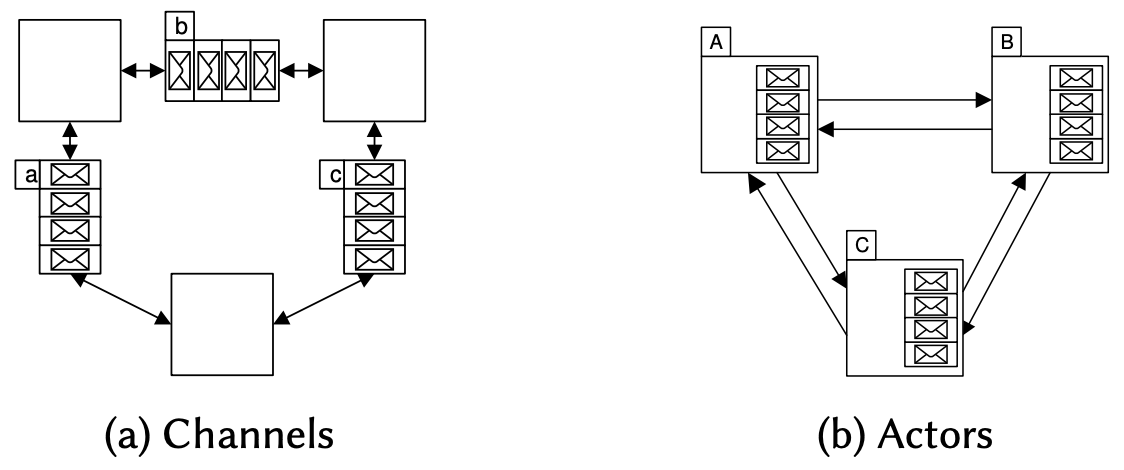
\includegraphics[width=0.7\linewidth]{images/channel_actor.png}    
    \caption{ (a) illustrates the Channels model with concurrent units communicating via message-passing channels. (b) shows the Actors model where each Actor independently processes messages from its queue. (\cite{fowler_mixing})
    }
    \label{fig:channel_actor} 
\end{figure}

\subsection{Pat's Solution}
To cope with these challenges, the introduction of Actor type systems has become an important advancement. In this context, the design of the Pat language introduces a new solution based on the Actor model along with a mailbox behavioural type system for the first time in a behavioural type system at the programming language level.


\section{Mailbox}
The mailbox communication mechanism is a core concept of concurrent programming widely used in a variety of programming environments, introduced by 
\cite{ford_1976_hardware}. It allows program components to exchange messages asynchronously, thus enabling efficient communication between processes or threads. And Erlang, as a language designed for concurrent and distributed programming, deeply integrates the mailbox communication mechanism as the cornerstone of its inter-process communication.

The Listing \ref{lst:erlangExample} is a concrete example of the application of the mailbox communication mechanism in Erlang: an asynchronous task processing model. In this model, the \textbf{empty\_task} function is a standby process that performs an asynchronous computation by receiving a message containing a Result. When the computation is complete, the Result is passed to the \textbf{queryable\_task} function. The function is in a waiting state, ready to respond to the client's query request and by sending the result of the computation back to the requester. In addition, it handles error status and returns an error if the computation request is received again. The client starts the asynchronous task through the client function, first creating a new process to run \textbf{empty\_task} through spawn, then sending computation commands and query commands to the process, and eventually receiving and printing out the results of the computation.

However, it also reveals some potential problems, such as the risk of self-deadlock. Self-deadlock occurs when a process waits for an event that will never occur, causing the process to hang permanently. In this example, if the AsyncTask process fails to receive any kind of query request after completing a computation task, possibly due to a client failure or logic error that did not send a query message, the \textbf{queryable\_task} will wait indefinitely for the query request, resulting in wasted resources and potential system performance degradation. Additionally, if the client mistakenly sends the computation command again instead of the query command, although the program is designed to return an error, this does not elegantly address the problem of receiving the computation request again in the asynchronous task completion state, and may result in unnecessary error handling and resource usage.

\lstset{style=erlangstyle}
\begin{lstlisting}[caption={Asynchronous task handling and querying implemented in Erlang}, label={lst:erlangExample}]
empty_task() ->
    receive
        { compute, Result} -> queryable_task(Result)
    end.
    
queryable_task(Result) ->
    receive
        { query, Pid } -> 
            Pid ! { reply, Result },
            queryable_task(Result); 
        { compute, _ } -> erlang:error("Task already computed") 
    end.
    
client() ->
    AsyncTask = spawn(async_task, empty_task, []),
    AsyncTask ! { compute, 2 },
    AsyncTask ! { query, self() },
    receive
        { reply, Result } ->
            io:fwrite("Task result: ~w~n", [Result])
    end.
\end{lstlisting}

\subsection{Behavioural Type System}
As described in the book "Behavioral Typing: from Theory to Tools" written by \cite{gay_2017_behavioural}, the Behavioral Typing System provides an innovative solution to the typing problem. The system facilitates efficient cooperation patterns in distributed applications by regulating inter-component interactions through behavioral contracts as service-level protocols. By defining precise communication protocols (i.e., timing session types), the behavioral typing system is able to carefully control and manage the timing of inter-component interactions, effectively deal with concurrency and synchronization issues, and ensure the consistency and predictability of system behavior. In addition, the runtime monitoring mechanism of the behavioral typing system can detect and respond to abnormal behaviors in the system in real time, which significantly improves the reliability and security of the system.

Further, \cite{ancona_2016_behavioral} researchers point out that recent developments in behavioral type theory are applied to guarantee diverse correctness properties of large-scale communication-intensive systems. They explored ways to use behavioral types in conjunction with object-oriented programming. Overall, behavioral type systems have not only successfully solved the type problem, but also empirically supported the correctness, security, and maintainability of distributed systems through their application in a variety of programming languages and computing environments. This highlights the importance of behavioral type systems in contemporary software development, especially in building complex distributed application scenarios.

\subsection{Mailbox Type}
Mailbox types are an essential part of behavioral type systems, originally used in process algorithms to capture mailbox contents mainly in the form of exchanged regular expressions. Mailbox types were introduced by \cite{deaposliguoro_2018_mailbox} to enhance the message-passing mechanisms of programming languages based on the role model. In the Pat language, each actor's mailbox is defined in detail through type annotations that specify not only the types of messages that the mailbox can receive, but also contain expected behavioral patterns such as the order in which messages are sent and received. This fine-grained type annotation allows developers to perform strict type checking of message passing patterns to achieve precise control of complex communication behaviors, which significantly improves the type safety of concurrent programming and effectively avoids common concurrency problems such as violation of communication protocols and deadlocks.

The following code snippet(Listing \ref{lst:patexample2}) from Pat's program demonstrates the application of mailbox types in real-world programming.This code simulates the processing of asynchronous compute and query tasks by defining \textbf{emptyTask} and \textbf{queryableTask} functions, as well as a client function. Where \textbf{emptyTask} is a mailbox for an empty task that can receive one \textcolor{red}{Compute} message and multiple \textcolor{red}{Query} messages. Once a \textcolor{red}{Compute} message is received, the mailbox will call \textbf{queryableTask}. and \textbf{queryableTask} represents a mailbox that has already received a \textcolor{red}{Compute} message, and this mailbox can only receive multiple \textcolor{red}{Query} messages. In these definitions, \textbf{guard} expressions are used to monitor the mailbox self and perform the appropriate actions based on the type of message received. This pattern not only shows how mailbox types can be used in Pat to control the sending and receiving of messages, but also how Pat can use the type system to statically check the behavior of concurrent programs to ensure communication protocol compliance and program robustness.

\lstset{
    style=patstyle,
    literate={·}{{\textperiodcentered}}1}
\begin{lstlisting}[caption={Implementing Concurrent Program for Asynchronous Task Processing and Result Querying}, label={lst:patexample2}]
def emptyTask(self:EmptyTask):1 {
    guard self: Compute · *Query {
        receive Compute[result] from self -> 
            fullFuture(self, result)
    }
}

def queryableTask(self:Result:Int):1 {
    guard self: *Query{
        free -> ()
        receive Query[user] from self ->
            user ! Reply[Result];
            queryableTask(self,Result)
    }
}

def client():1 {
    let asyncTask = new in spawn emptyTask(asyncTask);
    let self = new in 
    asyncTask ! Compute[2];
    asyncTask ! Query[self];
    guard self: Reply[Result] from self ->
        free self;
        print(intToString(result))
}

\end{lstlisting}

\section{Implementation Strategies}

\subsection{Scheduling}
Scheduling in computing systems refers to the strategic scheduling and management of the order in which jobs are executed. This process is a high-level strategic decision making aimed at optimising processes and computational tasks in terms of time and resource allocation. In a concurrent environment, it is the responsibility of the scheduler to determine the timing of execution of each task to ensure that processor resources are used efficiently while minimising the task completion time. In distributed systems, the scheduler's responsibility extends to task allocation across different compute nodes, aiming to maximise the utilisation efficiency of each node in the network. Regardless of the type of system, the fundamental purpose of scheduling is to improve the overall throughput capacity of the system. In this framework, control flow management techniques, such as CPS and CEK, provide execution-level support and implementation mechanisms for scheduling, enabling scheduling policies to be applied more flexibly and efficiently to complex computing tasks and system architectures.

\subsection{CPS and CEK}
Continuation Passing Style (CPS) is a high-level control flow management technique that operates by explicitly passing the unexecuted portion of a program, called a "continuation". In the functional programming paradigm, this approach allows a function not to return a result directly, but to continue execution by accepting another function (i.e., a "continue") and passing it control. This style is inherently suited to implementing non-blocking and asynchronous operations, and provides a great deal of flexibility in modern programming. Although CPS elegantly handles asynchronicity and non-blocking operations, it introduces the need for concurrent multi-process control and complex communication patterns in concurrent and distributed system applications. However, CPS applications may make the code structure appear more complex and rigid, which not only challenges the readability of the programme but also increases the maintenance cost.

The Pat language, however, is dedicated to the problem of communication in concurrent and distributed systems, employing mailbox types as its core communication mechanism. In such systems, the communication process is often asynchronous, the order in which messages are delivered is uncertain, and multiple concurrent senders and receivers may be involved. In contrast to CPS, CEK-style abstract machines provide a more detailed division of programme state - Continuation, Environment and Control - through more detailed Explicit management provides a more structured and flexible framework for dealing with such complex communications. In the context of Pat language applications, where nested evaluation contexts and aliasing issues need to be considered, the CEK machine demonstrates excellent adaptability and handling capabilities, making it ideal for supporting the features of the Pat language.

\subsection{Implementing Pat in OCaml}
OCaml was chosen as the implementation language for the Pat language primarily because of its excellent capabilities in functional programming. OCaml's strong type system and pattern matching capabilities provide an intuitive and flexible approach to data processing and control flow, greatly simplifying the implementation of language features. While languages like Rust also place a high value on efficiency and safety, OCaml's unique functional programming paradigm relies much less on mutable state, and this preference for immutability effectively reduces side effects, making concurrent programming safer and easier to understand. As a result, OCaml is particularly well suited to the development of systems such as compilers and language processors that require a high degree of reliability and clear logic.


%==================================================================================================================================
\chapter{Requirements}

The purpose of this chapter is to provide a comprehensive requirements analysis of the project, including explicit functional and non-functional requirements. The detailed description of the project's core components provides clear guidance for the design and implementation of the project, ensuring that the final product will meet the intended quality standards and performance metrics.

\section{Functional Requirements}
In terms of functional requirements, we focus on the core functions that must be implemented by the interpreter, including syntax parsing, program state control, task scheduling, and memory management, to ensure the basic operation and execution efficiency of the interpreter.

\subsection{Must Have}
\textbf{Grammar parsing capability}: Must be able to accurately parse all the syntactic structures of the Pat language, including but not limited to variable declarations, control flow statements (e.g., if-else, switch), as well as support for basic data types (integers, strings).

\textbf{Mailbox processing}: Realize the creation of mailboxes, message insertion, storage, retrieval and release functions.

\textbf{Program state control}: Adopts CEK machine to achieve precise control of the execution state of the Pat program to ensure the correct execution of program logic.

\textbf{Task Scheduling}: Implements a round-robin-based task scheduling mechanism to achieve fair task scheduling and support parallel task creation and execution.

\textbf{Memory management}: Integrate Garbage Collection mechanism to effectively manage memory usage and optimize resource utilization.

\subsection{Should Have}
\textbf{Execution flow printing}: In debug mode to provide the execution of step-by-step printing to assist developers to debug and understand the program execution process.

\textbf{Error Handling Mechanism}: Design and implement a well-defined error handling mechanism to effectively manage exceptions and runtime errors.

\subsection{Could Have}
\textbf{Garbage collection optimization}: Research and implement optimized garbage collection mechanism to reduce the impact of execution time and improve execution efficiency.

\textbf{Communication system enhancement}: Enhance the mailbox communication system to improve the efficiency and reliability of message delivery.

\subsection{Won't Have}
\textbf{Scheduling Algorithm Research}: Does not delve into other scheduling algorithms that might replace the polled scheduling approach such as EIO that has the capability of parallel IO operations. in order to focus on optimization of the current implementation.

\section{Non-Functional Requirements}
Non-functional requirements relate to the usability, and cross-platform compatibility of the interpreter to ensure that the interpreter not only meets the requirements in terms of functionality, but also provides a good user experience during use.

\subsection{Must Have}
\textbf{Cross-platform compatibility}: The interpreter should be able to run seamlessly on major operating systems including Windows, Linux, macOS to ensure wide availability.

\subsection{Should Have}
\textbf{Ease of use}: Design the interpreter to be friendly to novice users so that users can get started quickly.

\subsection{Won't Have}
\textbf{IDE Integration}: Plug-in support for popular IDEs (e.g. VS Code, IntelliJ) including syntax highlighting, code auto-completion, and quick jumps to definitions is not provided at this stage.

\textbf{Debugging tools integration}: Not integrated debugging tools , including the lack of support for breakpoint settings , single-step execution and variable status view function .


%==================================================================================================================================
\chapter{Design}

\section{Principles of CEK-style Machine}

\subsection{\texorpdfstring{$\lambda$}{lambda}-Calculus}
Before delving into the implementation and optimization of CEK machines, it is crucial to understand the underlying concepts and principles of $\lambda$-Calculus, a formal system for representing the logic of a computational process or mathematical function, introduced by mathematician Alonzo Church in the 1930s, which is one of the core foundations of modern computer science. The system focuses on the process of binding and substitution of variables and serves as a generalized model of computation, equivalent to a Turing machine, that exhibits the fundamentals of the theory of computation.

\begin{figure}[h]
    \centering
    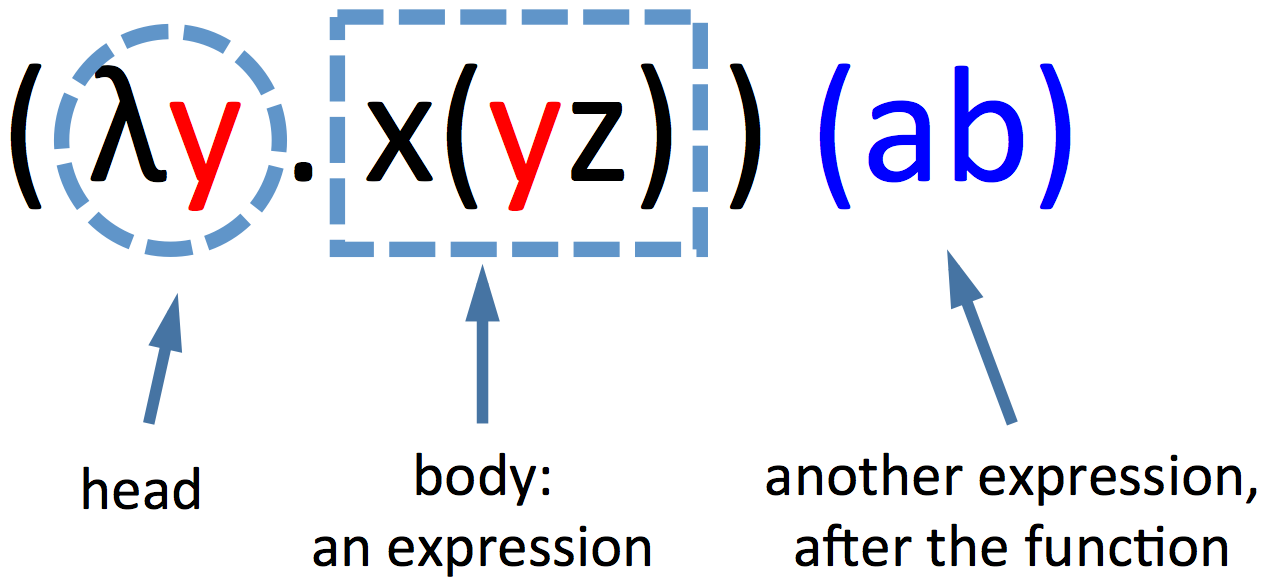
\includegraphics[width=0.35\linewidth]{dissertation/images/lambda1.png}    
    \caption{Illustration of $\lambda$-Calculus expression, showcasing the head of the expression marked in red, the body of the expression in dashed blue, and another expression following the function in solid blue (\cite{a2015_the})}
    \label{fig:lambda} 
\end{figure}

In the $\lambda$-Calculus system, all functions are defined anonymously, and their definition and application are accomplished uniquely through $\lambda$-abstraction. $\lambda$-expressions essentially define a function, which is realized by binding variables and expressing the expression inside the function body. The application of the function then simply places the actual arguments after the function name, without the need to separate them with parentheses or commas(Figure \ref{fig:lambda}). For example, Consider the $\lambda$-expression for a function that adds two numbers:
\[
\lambda x.\lambda y.x+y
\]
This expression is made up of two lambda abstractions:
\begin{itemize}
    \item $\lambda x$ which creates a function that takes an argument $x$
    \item $\lambda y$ which creates a function that takes an argument $y$
\end{itemize}
When this function is applied to two numerical arguments, such as 3 and 2, the operation proceeds as follows:
\begin{align*}
\text{Apply the first number: } & (\lambda x.\lambda y.x+y)3 \rightarrow \lambda y.3+y \\
\text{Apply the second number: } & (\lambda y.3+y)2 \rightarrow 3+2 \\
\text{Evaluate the addition: } & 3+2 \rightarrow 5
\end{align*}
Hence, the application of the lambda function \(\lambda x.\lambda y.x+y\) to the arguments 3 and 2 yields the result 5, which demonstrates basic function creation and application in lambda Calculus.

\subsection{Traditional CEK Machine}

The CEK machine, developed by \cite{felleisen_1986_control}, is a machine for $\lambda$-Calculus that is particularly well suited for describing and enforcing the semantics of functional programming languages. This machine, with its realism and abstraction, provides a framework to show how computers can efficiently execute programs. The basic CEK machine is based on a ternary configuration of the form $ \langle \ C\:|\:E\:|\:K \ \rangle $. where
\begin{itemize}
    \item $\textbf{C}$ for Control, the expression currently being evaluated;
    \item $\textbf{E}$ for Environment, binding free variables;
    \item $\textbf{K}$ for Continuation, which guides the action taken by the machine after completing the evaluation of the current term $C$.
\end{itemize}
Let us consider an expression "let $x$ = 3 in $x$ + 2". On this occasion we will execute it using the CEK machine:
\begin{align*}
& \left\{C: \textcolor{red}{\text{let } x = 3 \text{ in } x + 2}, E: \{\}, K: \text{empty}\right\} \\
\rightarrow & \left\{C: \textcolor{red}{3}, E: \{\}, K: \textcolor{red}{\text{let } x = [] \text{ in } x + 2}\right\} \\
\rightarrow & \left\{C: \textcolor{red}{x + 2}, E: \{\textcolor{blue}{x: 3}\}, K: \text{empty}\right\} \\
\rightarrow & \left\{C: \textcolor{red}{5}, E: \{\textcolor{blue}{x: 3}\}, K: \text{empty}\right\}
\end{align*}
In the initial phase, the CEK machine sets the control section to the full expression $\color{red}{\text{let } x = 3 \text{ in } x + 2}$. At this point, the environment is empty, indicating that no variable binding has been evaluated yet, and the continue section is also empty, indicating that no further computations are waiting to be evaluated. Next, the CEK machine recognizes the variable binding action in the $\color{red}{\text{let}}$ statement and begins to add the variable $\color{red}{x}$ to the environment in preparation for its association with the value $\color{red}{3}$. During this process, the control section is updated to $\color{red}{3}$, the environment is updated accordingly to contain the mapping $\color{blue}{\{x: 3\}}$, and the expression $\color{red}{x + 2}$ is placed in the continue section, waiting for a subsequent computation. When evaluating the computation of $\color{red}{x + 2}$, the CEK machine looks up and replaces the variable $\color{red}{x}$ with $\color{red}{3}$ in the environment, and then evaluates an addition operation to obtain the final result $\color{red}{5}$.

\subsection{Generalized CEK Machine}
In the design of the Pat language, reference was made to \cite{hillerstrm_2016_liberating}'s work on the generalization of the traditional CEK machine. This generalization process is particularly important for the Pat language because the traditional CEK machine was designed primarily for simple functional programming languages, which are overwhelmed when dealing with complex control flow and state management---especially algebraic effects. In the generalized CEK machine(Figure \ref{fig:equations}), the configuration takes the form of $\langle \boldsymbol{M}\: |\: \boldsymbol{\gamma} \:| \:\boldsymbol{\Sigma} \rangle$, where $\boldsymbol{M}$ represents the current term to be computed, which is equivalent to the control (C) part in the original CEK machine. $\boldsymbol{\gamma}$ represents the current environment, inherited from the environment (E) part in the original machine, which is in charge of binding the variables to the corresponding values. $\boldsymbol{\Sigma}$, on the other hand, represents the continuation part, which, unlike the continuation (K) of a single instruction or state in the original machine, consists of a series of continuation frames $[\boldsymbol{\delta}_1, \ldots , \boldsymbol{\delta}_n]$, each frame $\boldsymbol{\delta} = (\boldsymbol{\chi}, \boldsymbol{\gamma}, \boldsymbol{M})$ representing a pure continuation within a particular processor closure. Here $\boldsymbol{\chi}$ denotes the processor closure (handler closure), $\boldsymbol{\gamma}$ maintains its role as an environment for mapping variables to their values, and $\boldsymbol{M}$ represents the current computational term or expression being evaluated. 
\begin{align*}
\text{ Configurations}\;\; & C ::= \langle M \, | \, \gamma \, | \, \Sigma \rangle \\
\text{Environment}\;\; & \gamma ::= \cdot \, | \, \gamma, x \mapsto V \\
\text{ Frame stack}\;\; & \Sigma ::= \cdot \, | \, \sigma \circ \Sigma \\
\text{Frame}\;\; & \sigma ::= \langle \chi, \gamma, M \rangle \\
\text{Value}\;\; & v ::= \gamma(v) 
\end{align*}
\vspace{-2\baselineskip} 
\begin{figure}[ht]
    \caption{CEK Syntax}
    \label{fig:equations}
\end{figure}

With this design, even though \textbf{Yield} functionality is not usually provided directly in functional programming paradigms, the model effectively implements yield-like behavior. This is particularly important for thread scheduling in Pat. In a concurrent environment, \textbf{Yield} allows a thread to actively release processor resources, thus allowing the scheduler to allocate resources to other threads or tasks. The continuation part of the generalized CEK machine $\boldsymbol{\Sigma}$ provides the basis for implementing this operation. Each continue frame can be thought of as a pause point that contains all the information needed to resume execution, similar to the pause and resume mechanism of the yield operation.

Let us execute the expression again: let x = 3 in x + 2, this time with a generalized CEK machine:
\begin{align*}
& (M: \textcolor{red}{\text{let } \ x\ =\ 3\ \text{in } \ x\ +\ 2}, \gamma: \{\}, \Sigma: \text{empty}) \\
\rightarrow & (M: \textcolor{red}{3}, \gamma': \{\}, \Sigma: \langle M: \textcolor{red}{x}, \gamma: \{\}, (\textcolor{red}{x+2})\rangle \cdot \Sigma) \\
\rightarrow & (M: \textcolor{red}{x\ +\ 2}, \gamma: \{ \textcolor{blue}{x} \mapsto \textcolor{blue}{3}\}, \Sigma: \text{empty}) \\
\rightarrow & (M: \textcolor{red}{\text{\textlbrackdbl} x \text{\textrbrackdbl}}_{\gamma} + \textcolor{red}{2}, \gamma: \{ \textcolor{blue}{x} \mapsto \textcolor{blue}{3}\}, \Sigma: \text{empty}) \\
\rightarrow & (M: \textcolor{red}{3\ +\ 2}, \gamma: \{ \textcolor{blue}{x} \mapsto \textcolor{blue}{3}\}, \Sigma: \text{empty}) \\
\rightarrow & (M: \textcolor{red}{5}, \gamma: \{ \textcolor{blue}{x} \mapsto \textcolor{blue}{3}\}, \Sigma: \text{empty})
\end{align*}

Included in its initial state are the entire expression as the machine state \(M\), an empty environment \(\gamma\) indicating that there are no variables bound, and an empty stack \(\Sigma\) implying that there are currently no computations to be executed. This setup is similar in nature to a traditional CEK machine. However, as the evaluation process unfolds, the machine state is first updated to {\color{red}3}, signaling that the variable $\color{red}x$ is about to be bound to it, and simultaneously pushing the expression $\color{red}x + 2$ onto the stack, awaiting further computation. The role of the stack in this step is to hold the current computational context, including variables and environment, which is very different from the traditional CEK machine that simply puts the expression to be continued into the "continue" section.

Subsequently, when the machine state changes to $\color{red}x + 2$, the environment is updated to $\color{blue}x \rightarrow 3$, which shows that $\color{red}x$ has been successfully bound to {\color{red}3}. At this point, the stack is cleared, indicating that the system is ready to execute the expression. Next, the machine state expression $\color{red}\text{\textlbrackdbl} V \text{\textrbrackdbl}_{\gamma} + 2$ is computed by looking up in the environment and replacing $\color{red}x$ with {\color{red}3}, which in turn is transformed to {\color{red}3} + {\color{red}2}. Eventually, the machine status is updated to {\color{red}5}, signaling that the computation has been successfully completed. This example not only shows how the generalized CEK machine handles complex expressions and variable bindings but also highlights the importance of the stack in preserving execution context. 

\subsection{Operational Semantics}

The introduction of Environment is an essential improvement when exploring the operational semantics of the Pat language. In previous operational semantics design by \cite{fowler_2023_special}, the substitution of variables was usually accomplished through substitution operations, which required traversing the entire expression to replace all instances of the variable whenever a variable was used. This process is not only inefficient because it may involve multiple traversals of the entire expression tree, but it may also lead to the creation of multiple unnecessary copies. The introduction of environments optimizes this computational process and brings significant improvements at both theoretical and implementation levels.

As can be seen in Figure \ref{fig:Semantics}, the adopted generalized CEK machine makes important changes to the runtime syntax of the previous version, with environments forming part of the core composition, in a model in which environments are not just static structures storing variable bindings, but rather act as dynamic, queryable and updatable records, in stark contrast to the traditional substitution operation. contrasting with traditional substitution operations. Specifically, an environment ($\gamma$) is defined as a possibly empty sequence in which each entry is associated with a mapping from a variable to its value. Where "$\cdot$" denotes an empty environment, "$\gamma, x \mapsto V$" denotes an extended environment that maps the variable $x$ to the value $V$ on top of the existing environment $\gamma$.

In the Reduction rules section it can be seen that the environment component plays a key role. For example, in the E-APP rules, the computation of the function application $f(\overrightarrow V)$ involves retrieving the function definition from the environment and mapping the real parameter $\overrightarrow V$ to the formal parameter $\overrightarrow x$. This process again highlights the role of the environment in simplifying computation and improving efficiency.

\textbf{Runtime syntax}
\vspace{-\baselineskip} 
\begin{align*}
 \quad &\text{Runtime names} & a \quad & && \text{Guard contexts} \quad & \mathcal{G} ::=& \ \overrightarrow{G_1} \cdot [ \; ] \cdot \overrightarrow{G_2} \\
 \quad &\text{Names}        & u, v, w  & ::= x \mid a && \text{Configurations} & \mathcal{C}, \mathcal{D} ::=& \ \llparenthesis \ M, \gamma, \Sigma \ \rrparenthesis \mid a \leftarrow \textcolor{red!80!black}{\textbf{m}} [\overrightarrow{V}] \\
 \quad &\text{Environments} & \gamma  & ::=  \cdot \mid \gamma, x \mapsto V \quad  &&& \mid & \quad \mathcal{C} \ || \ \mathcal{D} \ | \ (va) \ \mathcal{C} \\
 \quad &\text{Frames}       & \sigma  & ::=  \langle x,\gamma, M \rangle && \text{Runtime type envs} & \Delta  ::=& \ \cdot \mid \Delta, u : T \\
 \quad &\text{Frame stacks} & \Sigma  & ::= \epsilon \mid \sigma \cdot \Sigma &&&& \fbox{%
    $ \mathcal{C} \longrightarrow{} _\mathcal{p}\mathcal{D}$
}
\end{align*}
\vspace{-0.5\baselineskip} 
\textbf{Reduction rules}
\begin{align*}
\quad & \text{E-LET} &  \quad \llparenthesis \ \textbf{let} \ x: T = M \textbf{ in } N, \gamma, \Sigma \ \rrparenthesis & \quad \longrightarrow  \quad \llparenthesis \ M, \gamma, \langle x, \gamma, N \rangle \cdot \Sigma \ \rrparenthesis \\
\quad &\text{E-RETURN} & \quad \llparenthesis \ V, \gamma', \langle x, \gamma, M \rangle \cdot \Sigma \ \rrparenthesis & \quad\longrightarrow  \quad \llparenthesis \ M, \gamma[x \mapsto V], \Sigma \ \rrparenthesis \\
\quad &\text{E-APP} & \quad \llparenthesis \ f(\overrightarrow{V}),\gamma, \Sigma \ \rrparenthesis & \quad\longrightarrow  \quad \llparenthesis \ M, \gamma[\overrightarrow{x} \mapsto \overrightarrow{V}], \Sigma \ \rrparenthesis \quad \\ 
&&& \quad \quad \quad \quad  ( \text{if } \mathcal{P} (f) = \textbf{def } f(\overrightarrow{x : A} ) : B \{ M \} )\\
\quad &\text{E-NEW} & \quad \llparenthesis \ \textbf{new}, \gamma, \Sigma \ \rrparenthesis & \quad \longrightarrow  \quad (va) (\llparenthesis  \ a, \gamma, \Sigma \ \rrparenthesis) \quad (a \text{ is fresh}) \\
\quad & \text{E-SEND} & \quad \llparenthesis \ a \ ! \ \textcolor{red!80!black}{\textbf{m}} [\overrightarrow{V}], \gamma, \Sigma \ \rrparenthesis & \quad\longrightarrow  \quad \llparenthesis \ (), \gamma, \Sigma \ \rrparenthesis \parallel a \leftarrow \textcolor{red!80!black}{\textbf{m}}[\overrightarrow{V}] \\
\quad &\text{E-SPAWN} & \quad \llparenthesis \ \textbf{spawn } M, \gamma,\Sigma \ \rrparenthesis & \quad \longrightarrow  \quad \llparenthesis \ (), \gamma, \Sigma \ \rrparenthesis \parallel \llparenthesis \ M, \gamma , \varepsilon \ \rrparenthesis \\
\quad &\text{E-FREE}&  \quad  \ (va)(\llparenthesis \ \textbf{guard } a: E \{ \mathcal{G}[\textbf{free } \mapsto M]\}, \gamma,\Sigma \ \rrparenthesis ) & \quad \longrightarrow \quad \llparenthesis \ M, \gamma, \Sigma \ \rrparenthesis \\ 
\multicolumn{4}{l}{\quad \text{E-RECV} \quad $\llparenthesis$ \ \textbf{guard } a: E \{ G[\textbf{receive } \textcolor{red!80!black}{\textbf{m}}[$\overrightarrow{x}$] \textbf{ from } y $\mapsto$ M]\}, $\gamma$, $\Sigma$ \ $\rrparenthesis$ $\parallel$ a $\leftarrow$ \textcolor{red!80!black}{\textbf{m}} [$\overrightarrow{V}$] \quad } \\
\multicolumn{4}{r}{$\longrightarrow$ \quad $\llparenthesis$ \ M, $\gamma$[$\overrightarrow{x}$ $\mapsto$ $\overrightarrow{V}$, y $\mapsto$ a ], $\Sigma$ \ $\rrparenthesis$ \quad \quad \quad }
\end{align*}
\vspace{-1.5\baselineskip} 
\begin{align*}
 \text{E-N}\text{\scriptsize U} \ \frac{\mathcal{C} \longrightarrow \mathcal{D}}{(va)\mathcal{C} \longrightarrow (va)\mathcal{D}} \quad \quad \text{E-P}\text{\scriptsize AR} \ \frac{\mathcal{C} \longrightarrow \mathcal{C'}}{\mathcal{C} \parallel \mathcal{D} \longrightarrow \mathcal{C'} \parallel \mathcal{D}} & \quad \quad \text{E-S}\text{\scriptsize TRUCT} \frac{\mathcal{C} \equiv \mathcal{C'} \ \ \mathcal{C'} \longrightarrow \mathcal{D'} \ \ \mathcal{D'} \equiv \mathcal{D}}{\mathcal{C} \rightarrow \mathcal{D}} & & & \\
\end{align*}
\vspace{-3\baselineskip} 
\begin{figure}[ht]
    \caption{Pat Oprational Semantics}
    \label{fig:Semantics}
\end{figure}


\section{Pat Scheduling}
The generalized CEK machine provides an execution-level support and implementation framework for the scheduling mechanism of the Pat language.Pat chooses the Round-Robin scheduling mechanism as a fair scheduling strategy, which centers on ensuring that all threads are given an equal amount of processor time, thus preventing any thread from occupying CPU resources for a long period of time. In Pat, this mechanism is improved by changing the time to steps to ensure that all threads get the same number of evaluation steps. This strategy effectively prevents threads from waiting indefinitely after a message is delivered. Once the evaluation steps of a thread reaches the preset upper limit, the system will automatically switch to the next thread in the queue, which ensures the timeliness of message processing between threads and avoids the problem of message backlog.

Figure 4.3 shows a simplified example of the Pat scheduling mechanism, where the active steps of each process are represented by the length of the color slice, and different colored slice are used to distinguish between processes. In this model, the maximum value of the step slice is set to 2, which means that after any process executes two steps, the scheduler will force it to move to the next process. The diagram clearly shows the state of the four processes (P1 to P4) during the execution steps. Process P1 reaches the maximum step slice limit after two steps of execution. Process P2 still has one step left to complete after the second step, at which point the scheduling mechanism interrupts P2 and switches to the execution of P3. After P3 completes, the system returns to complete the remaining steps of P2. Finally, P4 is executed similarly to P1. This allocation model ensures that the processes are executed sequentially in a fixed number of steps, reflecting the fairness of the rotation scheduling strategy and ensuring that no process will monopolize the processor resources for a long time.

\begin{center}
\begin{tabular}{c|*{9}{p{0.5cm}}}
\rowcolor{white}
\multicolumn{1}{c|}{Process\textbackslash Step} & \multicolumn{1}{c}{1} &\multicolumn{1}{c}{2} &\multicolumn{1}{c}{3} &\multicolumn{1}{c}{4} &\multicolumn{1}{c}{5} &\multicolumn{1}{c}{6} &\multicolumn{1}{c}{7} &\multicolumn{1}{c}{8} &\multicolumn{1}{c}{9} \\ \hline
P1 & \cellcolor{blue!25} & \cellcolor{blue!25} & & & & & & & \\
P2 & & & \cellcolor{red!25} & \cellcolor{red!25} & & & \cellcolor{red!25} & & \\
P3 & & & & &\cellcolor{green!25} & \cellcolor{green!25} & & & \\
P4 & & & & & & & & \cellcolor{yellow!25} & \cellcolor{yellow!25} \\
\end{tabular} \\
\textit{\textbf{Figure 4.3:} Pat's Round-Robin Scheduling}
\end{center}


\section{Garbage Collection}

Garbage collection is a core feature of automatic memory management in programming languages, designed to identify and free memory that is no longer being used by a program. This mechanism is essential for preventing memory leaks, improving software performance, and avoiding problems such as memory exhaustion. Especially in managed languages such as OCaml, the garbage collection process of objects is mostly transparent, however, the unique semantic properties of the Pat programming language, in particular its unique '\textbf{Free}' guard condition, make it necessary to adopt a special garbage collection strategy. This strategy ensures that the release of a mailbox is triggered only when no process references the particular mailbox.

The garbage collection mechanism in the Pat language(Fig \ref{fig:gc1}), inspired by the Mark-and-Sweep and Reference Counting methods, has been improved to manage memory resources efficiently. In the context of the Pat language, garbage collection of mailboxes requires traversing the state to ensure that all potential references have been considered. When the system detects that a process needs to block - usually because it is guarding a mailbox and waiting for a message, the garbage collector initiates a state traversal. This traversal consists of examining the environment of all processes to determine if a reference to the mailbox exists. If it exists, the reference counting method adds a reference count to that mailbox in a dictionary structure. The maintenance of this reference count ensures that the mailbox will not be released while at least one process may access it in the future.

When subsequent checks require the same process to be blocked again, the garbage collector will act based on the reference count of the mailbox in the dictionary. If the reference count is greater than zero, the garbage collector will block the process without having to do a full traversal, which is a significant efficiency improvement. The garbage collector will only perform a further full traversal if the reference count goes to zero, i.e., if the mailbox is not referenced in any process environment. If the reference count of the mailbox is \textbf{still zero}, meaning that it is no longer being guarded or used by any process, the garbage collector releases (frees) the memory occupied by the mailbox.


\begin{figure}[h]
    \centering
    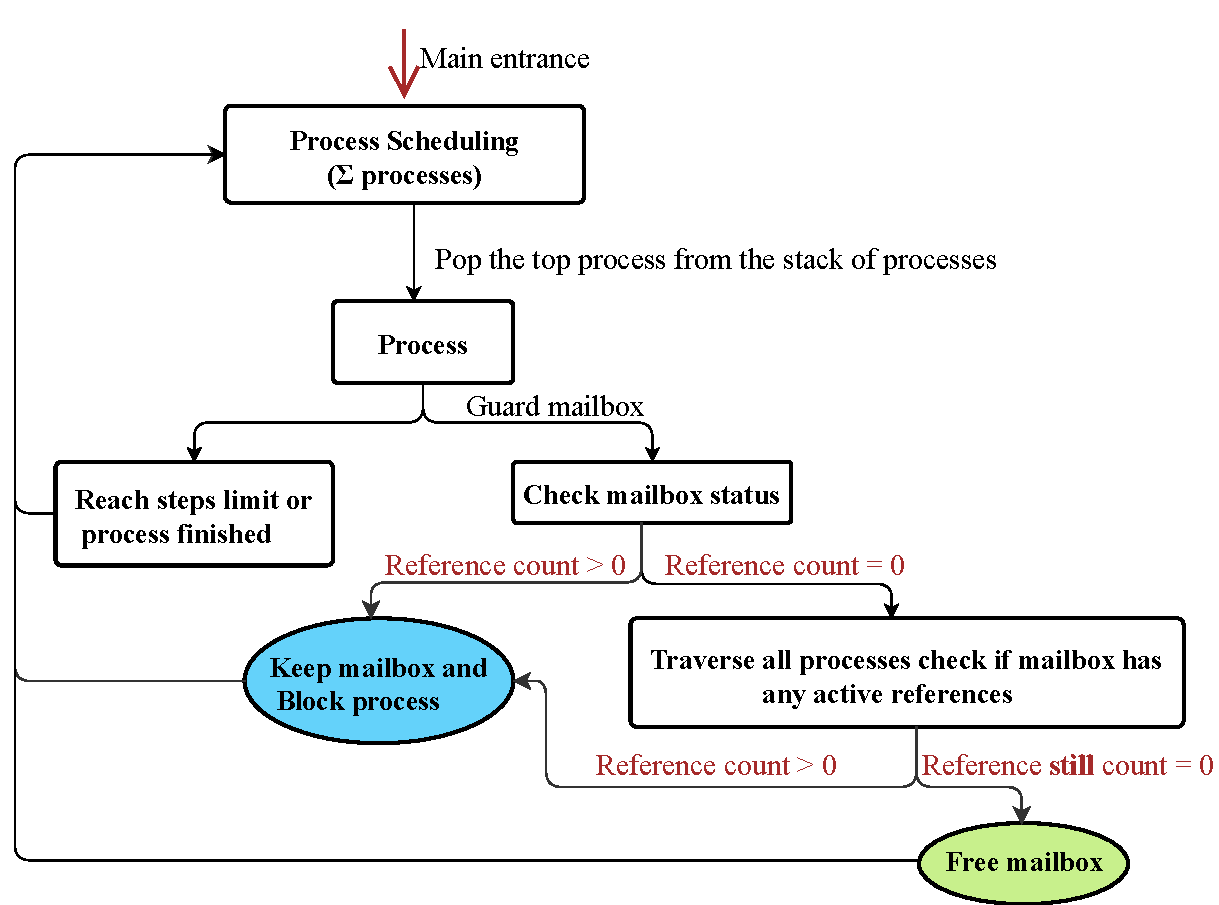
\includegraphics[width=0.8\linewidth]{dissertation/images/gc.pdf}    
    \caption{ 
    Garbage Collection Workflow in Process Scheduling
    }
    \label{fig:gc1} 
\end{figure}

In summary, the Pat language effectively manages memory resources by combining a garbage collection strategy with a similar idea of Mark-Sweep and Reference Counting methods, while avoiding the performance loading that frequent traversal may bring. The adoption of this strategy provides an efficient and safe solution for memory management in concurrent programming scenarios, guaranteeing the reasonable utilization of resources and stable execution of programs.




%==================================================================================================================================
\chapter{Implementation}


\section{CEK in Pat}
\subsection{Definition}
When implementing the Pat language interpreter based on the CEK machine, the main concern was to simulate the control flow in the execution of the program, the binding of environment variables, and the management of the continuation of the execution. Based on the source code provided by Listing \ref{lst:types}, we can see that processes are represented by tuples consisting of several components, including the entire \textbf{program}, \textbf{process ID}, the number of \textbf{steps}, the \textbf{computation expression}, \textbf{environment}, and the \textbf{frame stack}.

The \textbf{Control} in the CEK corresponds to the \textbf{comp} section of the code, which represents the currently pending computational expression. the \textbf{Environment} corresponds to the \textbf{(Ir.Binder.t * Ir.value)} list in the code, which is an environment list where each element is a binding that places a variable name. \textbf{Continuation} corresponds to the code's \textbf{frame list}, which is a frame stack in which each frame is a three-part tuple containing a variable binding \textbf{(Binder.t)}, an environment (also a list of variable-to-value mappings), and a computational expression to be executed. 

This represents the framework for the concrete implementation of the CEK machine in the Pat language interpreter. According to this framework, all subsequent code of the interpreter will follow this structure for the evaluation and execution of the program, ensuring that each step of the computation will be in the correct context and that the program flow can be properly controlled according to the execution path.

\noindent\begin{minipage}{\linewidth}
\lstset{style=Ocamlstyle}
\begin{lstlisting}[caption={Source Code of CEK Framework in Pat}, label={lst:types}]
type process = program * pid * steps * comp * 
(*@\hfill@*)environment * frame_stack
and pid = int
and steps = int
and environment = (Ir.Binder.t * Ir.value) list
and frame = Frame of Binder.t * environment * comp
and frame_stack = frame list
\end{lstlisting}
\end{minipage}


\subsection{Implementation of Keywords}
Specifically, depicted in  Lising \ref{lst:framework} is a pre-constructed Abstract Syntax Tree (AST) for the Pat language, a structure that provides the underlying framework for the interpreter execution discussed in the current dissertation. In this syntax tree, the evaluation of all keywords is realized through the CEK mechanism. Such as the \textcolor{red}{Return} keyword that marks the end of a computation, while \textcolor{red}{Let} and \textcolor{red}{LetPair} are concerned with variable binding and scope management, keeping the environment consistent. Composite structures such as \textcolor{red}{Seq} and \textcolor{red}{Case} show how the interpreter handles sequential and conditional branching, while \textcolor{red}{App} demonstrates the handling of function applications. More advanced control structures, such as \textcolor{red}{Spawn} and \textcolor{red}{Send}, deal with concurrency and message passing, showing how the interpreter operates within a broader model of computation, while \textcolor{red}{Guard} expressions allow for pattern matching as messages arrive, and are key to synchronization and communication in concurrent programming. As for \textbf{value}, it includes various data types such as \textcolor{red}{Constants},\textcolor{red}{Variables}, functions (via the \textcolor{red}{Lam} keyword), and \textcolor{red}{Mailbox} specialized for messaging, which are the elements that form the basis of program execution. This implementation ensures that the execution of the program not only follows the semantics, but also maintains the precision and consistency of the execution. Building on the above, the later parts of this chapter details the inner workings of some key mechanisms, including how the \textcolor{red}{Spawn} keyword supports process spawning, how the \textcolor{red}{Mailbox} enables efficient communication between processes, and how garbage collection is performed to optimize memory usage. The implementation of these mechanisms is critical to understanding the concurrent programming model and how the Pat language manages resources and synchronizes processes.

% \noindent\begin{minipage}{\linewidth}
% \lstset{style=Ocamlstyle}
% \begin{lstlisting}[caption={Source code for the specific implementation of evaluation for all keywords in Pat using the CEK architecture}, label={lst:framework}]
% match comp, env, stack with
% | Return _, _, [] -> ...
% | Annotate (term, _), env, stack 
% | Let {binder; term; cont}, env, stack 
% | LetPair {binders; pair; cont}, env, stack 
% | Seq (comp1, comp2), env, stack 
% | Return v, env, Frame (x, env', cont) :: stack
% | App {func; args}, env, stack
% | If {test; then_expr; else_expr}, env, stack
% | Case {term; branch1; branch2}, env, stack 
% | New interface_name, env, Frame (v, _, cont) :: stack
% | Spawn comp, env, stack
% | Send {target; message; _}, env, stack
% | Guard {target; pattern; guards; _}, env, stack
% \end{lstlisting}
% \end{minipage}

\noindent\begin{minipage}{\linewidth}
\lstset{style=Ocamlstyle}
\begin{lstlisting}[caption={AST in Pat}, label={lst:framework}]
type program = {
    prog_interfaces: Interface.t list;
    prog_decls: decl list; prog_body: comp option}
and decl = {
    decl_name: Binder.t; decl_parameters: (Binder.t * Type.t) list;
    decl_return_type: Type.t; decl_body: comp}
and comp =
    | Annotate of comp * Type.t
    | Let of {binder: Binder.t; term: comp; cont: comp}
    | Seq of (comp * comp)
    | Return of value
    | App of {func: value; args: value list}
    | If of { test: value; then_expr: comp; else_expr: comp}
    | LetPair of {binders: (Binder.t * Binder.t); 
                       pair: value; cont: comp}
    | Case of {term: value; branch1: (Binder.t * Type.t) * comp; 
                                    branch2: (Binder.t * Type.t) * comp}
    | New of string
    | Spawn of comp
    | Send of {target: value; message: message; 
                   iname: string option}
    | Guard of {target: value; pattern: Type.Pattern.t;
                    guards: guard list; iname: string option}
and value =
    | VAnnotate of value * Type.t
    | Constant of constant
    | Primitive of string
    | Variable of Var.t * Pretype.t option
    | Pair of value * value
    | Inl of value
    | Inr of value
    | Lam of {linear: bool; parameters: (Binder.t * Type.t) list;
                 result_type: Type.t; body: comp}
    | Mailbox of RuntimeName.t
and message = (string * value list)
and guard =
    | Receive of {tag: string; payload_binders: Binder.t list;
                       mailbox_binder: Binder.t; cont: comp}
    | Free of comp
    | Fail

\end{lstlisting}
\end{minipage}

% \subsection{Case Study}
% We may demonstrate the specific execution process and the value seeking strategy by means of an example. Below is a description of the two keywords Let and App for evaluating values in execution(Listing \ref{lst:letapp}). In the Pat language, the \textcolor{red}{Let} expression allows us to bind the result of an expression to a variable so that it can be used in subsequent computations. When this expression is encountered, we create a new \textcolor{darkgreen}{Frame} that contains the variable binders, the current environment, and the continuation body. We then recursively execute the bound expression \textbf{term}.

% \noindent\begin{minipage}{\linewidth}
% \lstset{style=Ocamlstyle}
% \begin{lstlisting}[caption={Let and App Keyword Specific Implementation}, label={lst:letapp}]
%     | Let {binder; term; cont},env,stack ->
%         execute (program,pid,steps+1,term,env,
%         (*@\hfill@*)(Frame (binder,env,cont)) :: stack)
%     | App {func; args}, env, stack -> 
%         (match func with
%             | Lam {parameters; body; _} 
%             | Primitive op
%             | Variable (func_var, _))
% \end{lstlisting}
% \end{minipage}

% If it is an \textcolor{red}{App} expression, the function will be applied to the arguments, and if the function is a lambda expression, a new environment will be created and bound to the arguments and the \textbf{Lambda} body will be executed recursively. For primitive operations such as \textbf{print}, \textbf{intToString}, etc., we will perform a specific evaluation strategy for each primitive and update the result buffer if necessary. As for ordinary functions, a lookup of the function definition will be performed, and if the corresponding function is found in the declaration of the program, the function body will be executed in the new environment \textbf{env'}. If a closure is found in the current environment, the corresponding function body is also executed. As a whole with these examples, it is shown how the CEK model handles different keywords in the Pat language and how the environment, stack, and continuation bodies are used to maintain program state during the value seeking process.

\section{Scheduler interaction}

In the implementation of Pat language, the core function of scheduler is introduced with the aim of providing an efficient and reliable concurrency mechanism for program running. Unlike the traditional round-robin scheduling mechanism based on time slices, we adopt a rotation scheduling strategy based on evaluation steps in the Pat language. Instead of scheduling tasks in terms of time, this strategy rotates tasks based on the number of evaluation steps they have completed. And we limit the maximum number of evaluation steps to 30. This is mainly for preliminary testing purposes, and aims to balance the execution efficiency and computational complexity of the language. It should be clear that this limit is not fixed, but is an adjustable parameter. As the language is further developed and application scenarios are expanded, this limit will be adjusted according to specific needs.

In the code shown on Listing \ref{lst:Scheduler}, the process\_scheduling function takes two arguments: \textbf{processes} is a list containing all the process to be executed, and \textbf{max\_steps} is the maximum number of steps each process is allowed to execute before being suspended. The logic of the function starts with a pattern match against the processes list. If the list is empty, all processes have been completed, which means the function is over. Otherwise, it takes the first process from the list and checks to see if the process has reached or exceeded its maximum number of allowed steps. If so, the process will be placed back at the end of the list and the number of steps reset to 0 so that it can be scheduled again later. If the process has not reached its maximum number of steps, it will be executed via the execute function. Execute returns a tuple containing the new \textbf{status} of the process and an \textbf{updated process}. Based on the status of the process after execution, the scheduler decides how to process next:

\begin{itemize}
\item $\textbf{Finished}$: If a process has completed, it is removed from the process list, and the scheduler proceeds to handle the remaining processes.
\item $\textbf{Unfinished}$: If a process is not finished(Reaching the maximum number of steps or other reasons), its updated state is appended to the end of the process list for future execution.
\item $\textbf{Spawned new\_process}$: If the execution spawns a new process (new\_process), this new process is added to the beginning of the process list, while the updated state of the current process is appended to the end.
\item $\textbf{MessageToSend (target, message)}$: If the current process needs to send a message to another process, the scheduler handles the message sending through the function.
\item $\textbf{Blocked need\_free\_check}$: If a process is blocked due to waiting for resources, some functions is responsible for managing the blocked state.
\item $\textbf{FreeMailbox mailbox}$: If a process releases a mailbox, the function takes care of the logic after freeing the mailbox.
\end{itemize}

Through this approach, the scheduler can effectively manage the execution of processes, concurrent spawning of processes, message passing, process blocking, and resource release, ensuring efficient system operation and rational resource allocation. The implementation of this scheduling strategy not only enhances the performance of concurrent programs but also achieves flexible adaptation to the varying computational demands of different tasks by dynamically adjusting the order and frequency of process execution.

\noindent\begin{minipage}{\linewidth}
\lstset{style=Ocamlstyle,}
\begin{lstlisting}[caption={Implementation of a round-robin scheduler based on evaluation steps in the Pat language}, label={lst:Scheduler}]
let rec process_scheduling processes max_steps =
  match processes with
  | [] -> ()
  | (prog, pid, steps, comp, env, stack) :: rest ->
     if steps >= max_steps then process_scheduling (rest @
     (*@\hfill@*)[(prog, pid, 0, comp, env, stack)]) max_steps
     else
       let (status, updated_process) = 
          execute (prog, pid, 0, comp, env, stack) 
       in
          match status with
          | Finished -> 
              process_scheduling rest max_steps
          | Unfinished -> 
              process_scheduling (rest @ [updated_process]) max_steps
          | Spawned new_process -> ...
          | MessageToSend (target, message) -> ...
          | Blocked need_free_check -> ...
          | FreeMailbox mailbox -> ...

\end{lstlisting}
\end{minipage}


\section{Case Study}

\subsection{Process Spawn}

Code snippet 1 in Listing \ref{lst:spawn} shows the specific code section that handles the generation of a new process by a process. When a \textcolor{red}{Spawn} operation is encountered, the system first generates a new process identifier(PID) through the \textbf{generat\_new\_pid()} function, which ensures that each generated PID is unique, incremented sequentially starting from 1, and ensures that the IDs of processes that have been marked as Finished are not reused. Subsequently, the newly created process is initialized with a new \textbf{PID}, a \textbf{step} reset to 0, and \textbf{comp}, \textbf{env}, and an \textbf{empty stack} inherited from the current process, as a way to ensure that the new process can continue to perform the computational tasks split from the current process. For the current process, its computation expression is updated to \textbf{Return (Constant Unit)}, which is designed to allow the current process to simply terminate its recursive execution early. This design ensures that the current process can quickly return to the scheduler, which in turn allows the scheduler to continue executing the newly spawned process.

In the process\_scheduling function depicted in Listing \ref{lst:Scheduler}, the returned Spawn state is precisely captured. At this point, the second code snippet in Listing \ref{lst:spawn} detailed this status, the scheduler places the newly spawned \textbf{new\_process} at the top of the process list by matching the state of the current process, while the current process, which failed to complete its execution, is relocated to the end of the process list. This operation ensures that the newly spawned process gets immediate scheduling so that it can start executing as soon as possible, and also ensures that the original process can continue executing in subsequent scheduling rounds if it has not completed its computational tasks. This mechanism ensures that every process gets scheduled at the right time, enabling efficient and fair resource allocation.

\noindent\begin{minipage}{\linewidth}
\lstset{style=Ocamlstyle,}
\begin{lstlisting}[caption={Process spawning mechanism in Pat}, label={lst:spawn}]
(*......*)
| Spawn comp, env, stack ->
    let new_pid = generate_new_pid () in
    let new_process = (program,new_pid, 0, comp, env, []) in
      Spawned new_process, (program, pid,steps+1, 
                                    Return (Constant Unit), env, stack)
(*......*)
| Spawned new_process -> 
    process_scheduling (new_process :: rest @ 
                                 [updated_process]) max_steps
(*......*)
\end{lstlisting}
\end{minipage}

\subsection{Mailbox Communication}
The mailbox communication feature is a key feature in the Pat language, providing an elaborate mechanism for inter-process message passing. This section describes the process of sending and receiving messages separately. 

\subsubsection{Sending Messages} \hfill\\\\
Listing Sending looks at how the send message operation is handled in the process. \textcolor{red}{Send} in the code snippet first constructs a \textcolor{red}{MessageToSend} status that includes the target mailbox variable (\textbf{target}), the message variable to be sent (\textbf{message}), and the actual value in its environment (\textbf{env}). It then updates the state of the current process by increasing its step count by one and updating the computational expression to \textbf{Return (Constant Unit)}, which indicates that the current process is expected to end its execution path.

Further, in the scheduler, the \textcolor{red}{MessageToSend} status is processed with the appropriate substitution and preparation of the destination address and message content via the \textbf{substitute\_in\_message} function to ensure that the message can be correctly sent to the specified mailbox. Afterwards, the \textbf{add\_message\_to\_mailbox} function is called to place the prepared message into the appropriate mailbox, and this operation may unblock the process waiting for the message on that mailbox. The scheduling process then proceeds with the remainder of the execution by rescheduling unblocked processes as a result of message reception into the execution queue, followed by placing the current process at the head of the list.

\noindent\begin{minipage}{\linewidth}
\lstset{style=Ocamlstyle,}
\begin{lstlisting}[caption={Message Sending in Pat}, label={lst:Sending}]
(*......*)
| Send {target; message; _}, env, stack ->
    (MessageToSend (target, message, env), (program, pid, 
  (*@\hfill@*)steps+1, Return (Constant Unit), env, stack))
(*......*)
| MessageToSend (target, ((tag, _) as message),env'') ->
    let _,messages = message in
    let (substituted_target, substituted_values) = 
    (*@\hfill@*)substitute_in_message env'' target messages 
    in let unblocked_process = add_message_to_mailbox 
    (*@\hfill@*)substituted_target (tag,substituted_values) pid 
    in process_scheduling ([updated_process] @ rest @ 
    (*@\hfill@*)unblocked_process) max_steps
(*......*)
\end{lstlisting}
\end{minipage}
 
\subsubsection{Receiving Messages} \hfill\\\\
In this receive message section(Listing \ref{lst:Guard}), when a process guards a mailbox, it first determines if the target is a Mailbox by using the \textbf{eval\_of\_var} function, and if it is, then it looks up the message list corresponding to the mailbox name. If a message exists in the corresponding message list, it iterates through the receive conditions defined in the guards. For each receive condition, check if there is a message in the message list that matches the condition. If it exists, the message is extracted, the message content is bound to an environment variable, and the corresponding continue expression (\textbf{cont}) is executed. If no matching message is found in the message list, the current process is marked as \textcolor{red}{Blocked}, indicating that it is waiting for a specific message to arrive.

\noindent\begin{minipage}{\linewidth}
\lstset{style=Ocamlstyle,}
\begin{lstlisting}[caption={Message Reception and Guard Evaluation in Pat Language}, label={lst:Guard}]
(*......*)
| Guard {target; pattern; guards; _}, env, stack ->
  (match pattern with  
    | Type.Pattern.One -> (* Free Mailbox *)
    | _ ->
      let need_free_check = (*......*) in
      let m = eval_of_var env target in
      match m with
        | Mailbox mailbox_name ->
            match Hashtbl.find_opt mailbox_map mailbox_name with
            | Some msg_list -> 
              let rec match_guards = function
                | Receive {tag; payload_binders; mailbox_binder; cont} 
                (*@\hfill@*):: rest ->
                    if (* tag = (tag in msg_list) *) then
                      let message_to_process = 
                          extract_message tag mailbox_name msg_list in
                      let new_env = bind_env message_to_process 
                      (*@\hfill@*)payload_binders env target mailbox_binder in
                      execute(program,pid,steps+1,cont,new_env,stack)
                    else
                      match_guards rest
                | [] -> 
                  (Blocked (need_free_check, mailbox_name), 
                              (program, pid, steps, comp, env, stack))
                | _ :: rest -> match_guards rest 
              in
              match_guards guards
(*......*)
\end{lstlisting}
\end{minipage}

\section{Execution of Garbage Collection Strategies}

In the Pat language, to implement its unique "Free" guarding feature, we use a garbage collection mechanism. This feature has three cases:

\begin{itemize}
\item When guard matches the pattern $\mathbb{1}$ or \textbf{Free V} appearing in the receive statement (which is syntactic sugar for the former), it means that the mailbox is empty, and therefore the mailbox can be freed directly. Specifically, according to Listing \ref{lst:Guard} when a match is made to \textbf{Type.Pattern.One}, the system returns \textcolor{red}{freeMailbox} (the message of the empty mailbox) to the scheduler. The first part of Listing \ref{lst:blockfree} shows the garbage collection process, in which all processes and references in their environments related to this mailbox are removed and the updated process is returned to the scheduler.

\item If the guard does not contain \textbf{Free V} or does not contain the pattern $\mathbb{1}$, the system will not perform a garbage collection operation (\textbf{need\_free\_check} is false in listing \ref{lst:Guard}), but instead, the process will be added directly in the scheduler to the \textbf{blocked\_list} and wait for further processing.

\item In addition to the above two cases, the system will perform the most important garbage collection check. When \textbf{need\_free\_check} is true, all processes will be traversed in \textcolor{red}{Blocked} status in the scheduler (second part of Listing \ref{lst:blockfree}) by \textbf{mailbox\_counting\_update}. Checks to see if a reference to a specific mailbox exists. If a reference exists, the mailbox counting is incremented and blocked on the next check. If still no reference is found, the same process as in the first case is performed.
\end{itemize}

\noindent\begin{minipage}{\linewidth}
\lstset{style=Ocamlstyle,}
\begin{lstlisting}[caption={Mailbox Free and Process Blocking}, label={lst:blockfree}]
(*......*)
| FreeMailbox mailbox -> 
    let new_processes = update_processes_after_free 
    (*@\hfill@*)(updated_process::rest) mailbox 
    in
    process_scheduling new_processes max_steps
| Blocked (need_free_check,mailbox)->
    let should_block = 
      if need_free_check then
        let all_processes = rest @
          (Hashtbl.fold (fun _ process acc -> process :: acc) 
          (*@\hfill@*)blocked_processes []) in
          if mailbox_counting_update mailbox all_processes then true
          else (* Still no reference, free mailbox *)
      else true
    in
    if should_block then
        add_process_to_blocked_list mailbox updated_process;
        process_scheduling rest max_steps
    else ()
(*......*)
\end{lstlisting}
\end{minipage}

\section{Evaluation Step Printer}

In order to achieve transparent observation during the evaluation process of the Pat language and to easily be debugged, this research implements a step printer whose core function is to capture and print the current execution state at each evaluation step. Specifically, by calling the \textbf{print\_config} function defined in Listing \ref{lst:Printer}, the current number of evaluation steps is first recorded via counter to allow for tracking the progress of the execution process. Next, the function constructs and splices the status strings of different components separately, including the identifier of the current process, the number of steps, the description of the computation expression, the environment variables, the contents of the execution stack, and the current status of the mailbox mapping and blocking processes. This mechanism not only provides developers with real-time execution feedback, but also greatly simplifies the debugging process and performance analysis by accurately displaying the state changes at each step. In addition, the listing shows that the printer will specifically label the states such as the end of the process and blocking, further increasing the visualization and readability of state changes. With these detailed outputs, it is easier to locate problems and optimize concurrency strategies and resource management.

\noindent\begin{minipage}{\linewidth}
\lstset{style=Ocamlstyle,}
\begin{lstlisting}[caption={Evaluation Step Printer}, label={lst:Printer}]
(*......*)
let print_config (comp, env, stack, steps, pid, mailbox_map, 
                         blocked_processes) =
  counter := !counter + 1;
  let step_str = Printf.sprintf "\n Total step %d\n" !counter in
  let mailbox_map = print_mailbox_map mailbox_map in
  let blocked_processes = 
          print_blocked_processes blocked_processes in
  let steps_str = Printf.sprintf "\n\nCurrent PID: 
  (*@\hfill@*)%s Steps: %d\n\n" string_of_int pid steps in
  let comp_str = Printf.sprintf "Comp: %s\n\n" (show_comp comp) in
  let env_str = Printf.sprintf "Env: %s\n\n" (show_env env) in
  let frame_stack_str = Printf.sprintf "Frame Stack: %s\n"
  (*@\hfill@*)(show_frame_stack stack) in
  step_str ^ mailbox_map^ blocked_processes ^ steps_str ^
                 comp_str ^ env_str ^ frame_stack_str
(*......*)
Buffer.add_string steps_buffer
         (Printf.sprintf "\n Process %d Finished \u{2705} \n" pid);
(*......*)
Buffer.add_string steps_buffer 
         (Printf.sprintf "\n Process %d Blocked \u{1F6AB} \n" pid);

\end{lstlisting}
\end{minipage}

Listing \ref{lst:output} shows a concrete example of the output of the step printer during the execution of the Pat language, where the output first shows the mailbox count status. This is followed by a detailed listing of the state of all mailboxes currently in the system, including mailbox identifiers (e.g., alice0, bob1, self2) and a list of the messages each contains. This section provides an intuitive view for understanding inter-process communication and is especially important when debugging message passing and synchronization issues. A list of currently blocked processes is also shown, including the mailboxes waiting for messages and their corresponding PIDs. this information helps developers to quickly identify potential deadlocks or resource contention problems. Finally, a full picture of the current execution context is provided, including inter-process function calls, variable bindings, and stack frame changes.

\noindent\begin{minipage}{\linewidth}
\lstset{style=printer,}
\begin{lstlisting}[caption={Example of Evaluation Step Printer Output}, label={lst:output}]
Mailbox_counting:
    Mailbox: self2, Value: 1
------------------- Total step 22 --------------------
Mailbox: alice0, Messages: [(Debit, [(Ir.Constant 
(*@\hfill@*)(Common_types.Constant.Int 20)),(Ir.Mailbox future3)]);]
Mailbox: bob1, Messages: []
Mailbox: self2, Messages: []
Blocked process:
   Mailbox: self2 -> PID: 1 
   Mailbox: alice0 -> PID: 2 
Current PID: 3 Steps: 2
Comp: Ir.App {func = (Ir.Variable (await4, (Some (Int, 
                             AccountMb!(Debit) [U]) -> FutureMb)));
                   args = [(Ir.Variable (amount29, (Some Int)));
                      (Ir.Variable (recipient28, (Some AccountMb)))]}
Env: [self30 -> Mailbox bob1; amount29 -> 20; recipient28 -> 
        Mailbox alice0; sender27 -> Mailbox self2; 
        self22 -> Mailbox bob1; balance21 -> 20]
Frame Stack: 
   [Frame(future,[self30->Mailbox bob1;amount29->20; 
            recipient28 -> Mailbox alice0; sender27 -> Mailbox self2]
\end{lstlisting}
\end{minipage}

\section{Error Handling Strategies}

During the development of the Pat language, in addition to enhancing debugging transparency through step printers, a set of error handling strategies were designed to ensure the maintainability of the program in case of runtime errors. The \textbf{failwith\_and\_print\_buffer} function, illustrated in Listing \ref{lst:error}, is the core of this strategy and is called when a runtime error such as "invalid configuration", "no mailbox matched" or "no free guard found" is encountered during program execution.

The logic of this function is to first call a series of print functions, these functions are responsible for the buffer accumulated in all the execution steps, process status and the results of the output, thus providing a detailed record of the execution of the track. By presenting this information, it is possible to quickly track down the specific step and context that triggered the error. In short, it provides effective support for handling complex error scenarios that are common in concurrent programming.

\noindent\begin{minipage}{\linewidth}
\lstset{style=Ocamlstyle}
\begin{lstlisting}[caption={Integrating Step Printing with Runtime Error Diagnosis.}, label={lst:error}]
(*......*)
let failwith_and_print_buffer msg =
  steps_buffer_print (); 
  process_buffer_print ();
  result_buffer_print ();
  failwith msg
(*......*)
| _ ->  failwith_and_print_buffer "Invalid configuration"
(*......*)
| None -> failwith_and_print_buffer "No mailbox matched"
(*......*)
| _ -> failwith_and_print_buffer "No free guard found")
(*......*)
\end{lstlisting}
\end{minipage}


%==================================================================================================================================
\chapter{Evaluation} 
In this research, we comprehensively evaluated the effectiveness of the Pat language runtime interpreter, employing methods such as correctness testing and micro-benchmarking, aiming to accurately quantify its performance metrics. Correctness testing ensured that the Pat language executed as expected when processing different example files, verifying the correctness of the language design and runtime. The efficiency of the interpreter in performing computationally intensive tasks was evaluated through careful measurements of the runtime of specific algorithmic tasks (e.g., computing Fibonacci series), and these tests focused on evaluating the performance of the Pat language under real-world running conditions. The tests were performed on a computer equipped with an M2 Pro chip and 16 GB of RAM, with the operating system MacOS 14.3, using the OCaml version 5.1.0 environment, and the time calculations, which included all parts of the type checking and the interpreter, were repeated 100 times, thus ensuring the accuracy and reliability of the results.

\section{Concurrent Reduction}

\subsection{Functional Reduction}
In performing a series of fundamental tests on the Pat language, we aim to verify whether the Pat language is able to accurately execute basic programming constructs and how well it performs in different programming scenarios. These tests help to evaluate whether the runtime environment of the Pat language can meet the needs of concurrent programming, and whether it can correctly handle various programming tasks according to its design specifications.

Specific tests performed include basic arithmetic tests, operator precedence, logical operation tests, anonymous functions, local variables and function bindings, empty interfaces and linear functions, type annotations, and pattern matching. The results of the tests show (Table \ref{tab:Fundamental_results}) that all tests were successfully completed as expected and no runtime errors were found. This result proves that the underlying functionality of the Pat language matches the design specifications and is capable of handling a wide range of programming tasks.

\begin{table}[ht]
\centering
\renewcommand{\arraystretch}{0.9}
\resizebox{\textwidth}{!}{%
\begin{tabular}{l l c c}
\toprule
\textbf{Name}  & \textbf{Description}   & \textbf{Exp.} & \textbf{Act.}  \\
\midrule
Arithmetic I  & Basic arithmetic check & True & True \\
Arithmetic II  & Operator precedence checks arithmetic order & True & True \\
Arithmetic III & Logic \& arithmetic test combines operations  & False & False \\
Anonymous Function & Function returns input integer value & 5 & 5 \\
Local Binding & 
Local binding and function definition & 10 & 10 \\
Nested Binding & Nested function returns double input value & 10 & 10 \\
Memory Management & Interface declaration and memory deallocation & ( ) & ( ) \\
Type annotations & Handles union type and printing & 5 & 5 \\
Pattern Matching & Pattern matching with union types & 5 & 5 \\
\bottomrule \\
\end{tabular}%
}
\caption{Functional Correct Test Results}
\label{tab:Fundamental_results}
\end{table}

\subsection{Concurrency Reduction}
After the functional correct tests were completed, we further tested the correctness of six advanced concurrency models for the Pat language, based on the original mailbox algorithmic model with ideas taken from the research of \cite{deaposliguoro_2018_mailbox}. The specific test implementations refer to the research of \cite{fowler_2023_special}. These test cases cover everything from concurrent lock, future variable handling, and account concurrent transactions, account concurrent transactions via future variables, master-worker parallel networks, and session-type communication actor models using a single arbiter.

First, we simulate concurrent locks to verify the efficiency and reliability of the Pat language in handling mutually exclusive operations. In addition, we evaluated the performance of the Pat language in handling one-time write and multiple read operations by testing the "Future" variable. Then, by simulating debit/credit instruction exchanges between concurrent accounts, we further validate the accuracy and efficiency of the Pat language in complex concurrency scenarios. In order to explore the application of Pat in asynchronous programming model, we also test the debit/credit commands of accounts implemented by "Future". In addition, we evaluate the performance of the Pat language by constructing a parallel network of master-worker jobs. Finally, we explore the ability of the Pat language to implement complex communication protocols through a session-type communication actor model, which involves the use of a single arbiter to coordinate communication behavior.

All tests show that the Pat language is able to successfully handle these high-level concurrent and programming tasks, fully indicating alignment between expected and actual output(Table \ref{Concurrency_result}). The test results not only validate the performance of the Pat language in different programming scenarios, but also demonstrate its power in handling concurrent system programming requirements. The average response times ranged from 45.8 ms for the concurrent model to 102.9 ms for the session type model, further proving that the Pat language is able to provide a high degree of functionality and reliability while ensuring performance.
\begin{table}[ht]
\centering
\renewcommand{\arraystretch}{1.1}
\resizebox{\textwidth}{!}{%
\begin{tabular}{l l c c}
\toprule
\textbf{Name}       & \textbf{Description}   & \textbf{Exp.}  & \textbf{Act.}\\
\midrule
Lock   & Concurrent lock modelling mutual exclusion       & 12 & 12  \\
Future  & Future variable that is written to once and read multiple times & 55         & 55          \\
Account             & Concurrent accounts exchanging debit and credit instructions  & ( ) & ( )                 \\
Account Future & Concurrent accounts where debit instructions are effected via futures  & ( ) & ( )                  \\
Master-Worker       & Master-worker parallel network            & 55385 & 55385                  \\
Session Types       & Session-typed communicating actors using one arbiter   & 6 & 6                 \\
\bottomrule \\
\end{tabular}%
}
\caption{Advanced Concurrency Model Correct Test Results}
\label{Concurrency_result}
\end{table}


\section{Micro-Benchmark Test}

Based on the correctness tests, we designed and implemented a series of benchmark tests aimed at evaluating the performance of the Pat language's runtime interpreter under different concurrent programming patterns. These tests cover a wide range of concurrent programming scenarios including master-worker (e.g., KFork, Fibonacci, Log Map), client-server (e.g., Ping Pong, Counter), and peer-to-peer (e.g., Big), and involve common network topologies such as Star (e.g. Philosopher, Smokers, Transaction) and Ring (e.g. Thread Ring), as referenced from part of the savina benchmarks written by \cite{imam_2014_savina}. Each test is designed to evaluate the execution efficiency of the Pat language under a particular concurrency model.

The purpose of these benchmarks is to establish an initial performance baseline for the Pat language and to demonstrate that it can effectively handle multiple concurrency models. Given that the Pat language is the first programming language to integrate mailbox typing, we do not use the results of these tests for direct comparisons with existing functional languages on the market. Instead, our goal is to demonstrate the controlled operation of the Pat language by showing how it can stably execute multiple concurrency patterns based on a design and implementation that incorporates the concept of mailbox types.

Through this series of benchmark tests, we observe the performance of the Pat language under different concurrency models (table \ref{Savina}). For example, the Ping Pong test evaluates the message processing speed by simulating the bidirectional delivery of messages; the Thread Ring test measures the message delivery latency by passing tokens in a ring network; and the Fibonacci test demonstrates the efficiency of the Pat language in handling recursive concurrency tasks. Note that in the Smokers test, this design caused a significant increase in test execution time due to the introduction of a randomized sleep function.

In tests performing the K-Fork model, the range of random numbers generated by the rand function in the initial code was too large, thus making the computation process excessively time-consuming. In light of this, we adjusted the upper limit of random numbers from 100,000 ms to 10 ms. This adjustment makes the computation process more efficient and more closely matches the lightweight computation needs of actors processing messages in real application scenarios. In addition, the initial code's multiple message flooding of a single mailbox (100, 1000, and 10000 messages, respectively) actually caused the mailbox to be overloaded. To more realistically simulate mailbox performance under regular load, we reduced the number of floods to a two and fixed the total number of messages to 20. These optimizations improve the accuracy and reliability of the benchmark in evaluating concurrent processing performance.

\begin{table}[ht]
\centering
\renewcommand{\arraystretch}{1.1}
\resizebox{\textwidth}{!}{%
\begin{tabular}{l l c}
\toprule
\textbf{Name} & \textbf{Description} & \textbf{Avg Time (ms)} \\
\midrule
Ping Pong & Process pair exchanging \( k = 5 \) ping and pong messages & 54.5 \\
Thread Ring & Ring network where actors cyclically relay one token with counter \( k = 1000 \) & 541.5 \\
Counter & One actor sending messages to a second that sums the count & 45.5 \\
K-Fork & Fork-join pattern where a central actor delegates \( k = 20 \) requests to workers & 76.2 \\
Fibonacci & Fibonacci server delegating parallel actors with \( k = 5 \) & 56.7 \\
Fib\_pairs & Fibonacci actors recursively resolving and returning terms independently & 55.1 \\
Big & Peer-to-peer network where actors exchange \( k = 100 \) messages & 265.8 \\
Philosopher & Dining philosophers problem & 111.9 \\
Smokers & Centralised network where one arbiter allocates \( k = 10 \) messages to actors & 5578.4 \\
Log Map & Computes the term \( xx + 1 = r \cdot xx \cdot (1 - xx) \) by delegating to parallel actors & 97.9 \\
\bottomrule \\
\end{tabular}
}
\caption{Part List of Savina Benchmarks}
\label{Savina}
\end{table}

In the field of concurrent computation, efficiently managing the overhead of parallel execution is one of the key factors in achieving high performance. By comparing the performance of these two strategies in computing Fibonacci series, we aim to evaluate the efficiency and feasibility of concurrent execution in the Pat language. We have chosen selected a range of K values (from 1 to 10) as input parameters to observe the variation of execution time for different input sizes. As shown in the figure \ref{fig:benchmark}, the graph on the left side demonstrates the comparative results of Fibonacci computational performance. The curves for sequential execution and concurrent execution closely follow each other, showing the similarity in time complexity between the two execution modes. Notably, Concurrent execution introduces no additional significant overhead, suggesting that the concurrency model of the Pat language has a potential advantage in maintaining low overhead.

In addition, we consider a Ping Pong performance test as an example of concurrent communication overhead. In this test, we only considered concurrent execution (without the sequential execution model) to demonstrate the linear relationship between execution time and input size. The graph on the right clearly depicts this relationship, a finding that suggests that in the Pat language, even in concurrent tasks that require frequent communication, the execution time remains linear, unaffected by significant concurrency overhead.

\begin{figure}
    \centering
    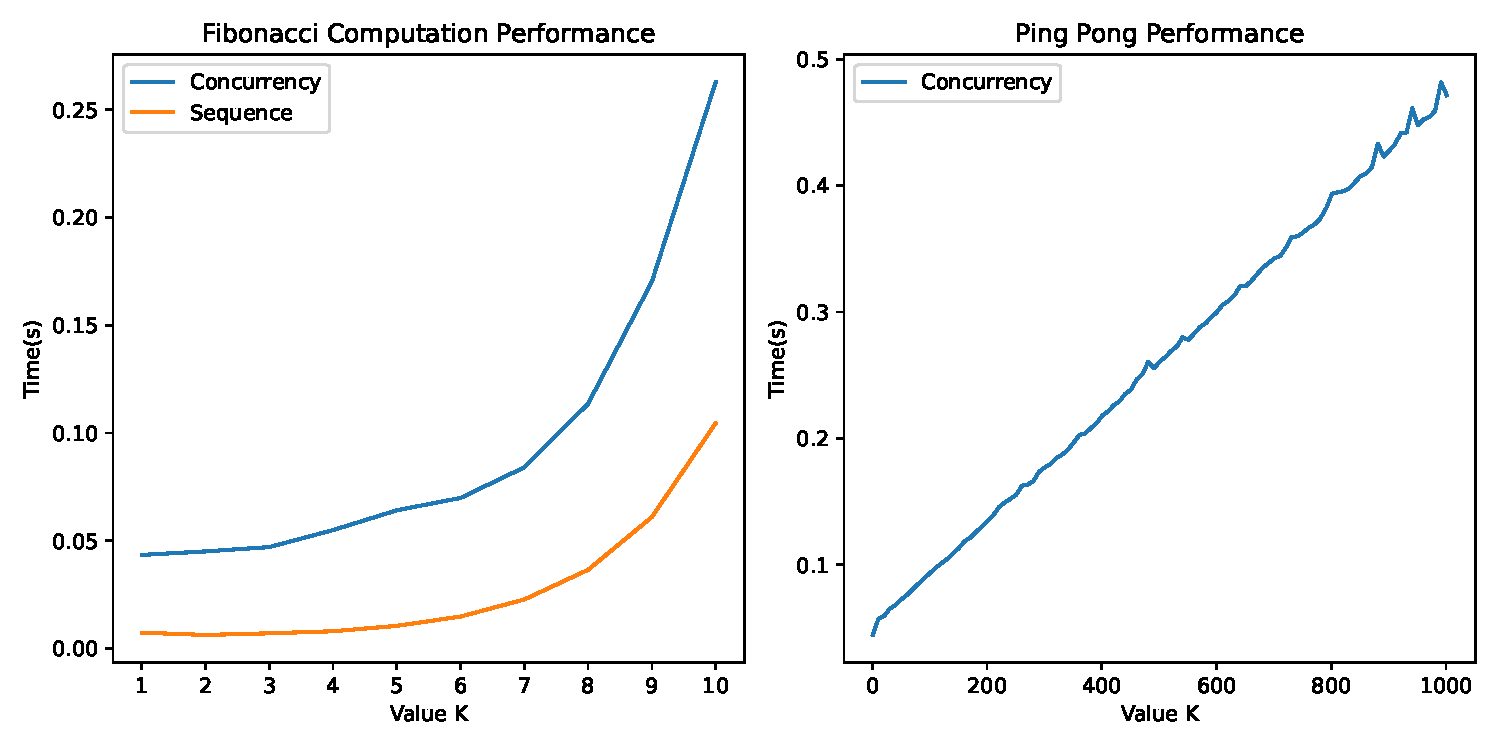
\includegraphics[width=0.88\linewidth]{dissertation/images/benchmark.pdf}    
    \caption{ 
    Comparative Execution Times of Sequential and Concurrent Code Snippets in Pat Language at Various K Values
    }
    \label{fig:benchmark} 
\end{figure}

In summary, these benchmark tests provide us with a comprehensive evaluation framework to scrutinize the performance of the Pat language in the area of concurrent programming. The unique advantages of the Pat language in handling complex concurrent tasks are demonstrated. This research provides important references and insights for the future development of functional language design and concurrent programming patterns for mailbox types.

\section{Reflection}
In the reflection section, the discussion of the research on garbage collection optimization and scheduling algorithms reveals two key areas in our research and development process, as well as pointing to potential directions for future work.

\subsection{Garbage Collection Optimization}

For garbage collection optimization section, we currently employ a mechanism that similarly combines a simple Mark-Sweep algorithm and a Reference Counting method. This approach provides our system with basic memory management capabilities. Although this combined strategy works effectively in many cases, we also recognize its limitations when dealing with branching statements such as if/switch, and complex programming constructs such as recursion. Especially in recursive calls and complex control flow structures, the simple reference counting method may not be able to accurately identify all garbage objects, resulting in memory not being reclaimed in a timely manner, thus affecting the execution efficiency and stability of the system.

Therefore, given enough time, we plan to explore and implement a deeper reference counting algorithm: Perceus, a precise reference counting method that combines reuse and specialization developed by \cite{reinking_2021_perceus}. This approach is mainly implemented by delaying the execution of the dup operation and executing the drop operation as early as possible. A dup operation here means increasing the reference count of an object, while a drop operation decreases the reference count. When the reference count drops to zero, the object is released.

In a traditional reference counting system, whenever a variable is copied, the dup operation is executed immediately to increase the reference count of the object. However, this immediate increase in the reference count may not always be necessary, especially if some variables are no longer needed in the short term.The Perceus algorithm increases the reference count by delaying the execution of the dup operation until the reference actually needs to be shared by multiple owners. This strategy reduces unnecessary reference count adjustments. In contrast to delaying execution of the dup operation, the Perceus algorithm performs the drop operation as early as possible. This means that as soon as it is determined that an object is no longer needed, its reference count is immediately reduced, and the object is also freed immediately if the reference count drops to zero. This approach optimizes memory utilization because it ensures that objects that are no longer needed are reclaimed in a timely manner.

In summary, Perceus provides an efficient reference counting mechanism that supports complex control flow and programming constructs through precise memory management, while reducing memory leaks and improving system performance. We therefore believe that Pat's memory management and stability can be significantly improved by introducing this innovative algorithm.

\subsection{Advanced Scheduling Methods}

Regarding the research on scheduling algorithms, our current implementation employs the Round-Robin scheduling approach, which is a simple and straightforward scheduling strategy. However, we also recognize that other framework, such as the \cite{_2024_ocamlmulticoreeio} scheduling, which is capable of supporting parallel IO operations, may provide better performance and efficiency(Figure \ref{lst:eio}).The introduction of EIO not only takes advantage of the high-performance IO operation features provided by modern operating systems, such as Linux's io\_uring, but also allows concurrent code to be written in a much more concise and efficient manner through a direct style of IO stacking. This approach does a lot more than just reduce heap allocation and increase speed, it also makes concurrent code written in the same style as non-concurrent code, which greatly improves the readability and maintainability of the code.

Within the time constraints of the project, we did not explore these alternatives in depth. Had we had more time, we would have compared the performance of different algorithms under multiple loads and scenarios, and we could have determined the scheduling strategy that best suited our system. In addition, research on how to combine multiple scheduling strategies in order to dynamically select the scheduling algorithm that best suits the current execution environment and task characteristics will also be a focus of our attention.

\noindent\begin{minipage}{\linewidth}
\lstset{style=ocamlstyle}
\begin{lstlisting}[caption={Example of running two threads of execution concurrently using Eio.Fiber}, label={lst:eio}]
let main _env =
  Fiber.both
    (fun () -> for x = 1 to 3 do traceln "x = %d" x; Fiber.yield () done)
    (fun () -> for y = 1 to 3 do traceln "y = %d" y; Fiber.yield () done);;
\end{lstlisting}
\end{minipage}


%==================================================================================================================================
\chapter{Conclusion}    

In this research, we explore the importance of concurrent and distributed systems in modern computational science. By comparing the concepts, challenges, and case studies related to concurrent programming and distributed systems, we propose a new programming language, the Pat language.The Pat language, by introducing advanced concurrent programming primitives and a unique mailbox type system, aims to provide developers with a more intuitive and concise way of handling concurrent tasks and communication processes. The goal of this research is to develop a runtime interpreter that specifically supports the Pat language, which not only needs to fulfill the runtime requirements of a general programming language, such as memory management, but also focuses on the specific needs of concurrent computation.

Starting from the foundations of concurrency and distributed systems, our research work provides an deep analysis of the main challenges facing concurrent programming in modern computing environments, such as thread deadlocks, communication mismatches, and data consistency problems. Through case studies, we demonstrate the value of concurrent programming in real-world applications such as multiplayer online game servers and so on. These case studies not only demonstrate the importance of concurrent programming in improving system throughput and response time, but also reveal the technical challenges faced in designing efficient and reliable concurrent systems.

To address these challenges, we have successfully implemented a runtime interpreter for the Pat language, whose main innovation is the introduction of a mailbox type system that statically constrains the order of message passing and processing through a type-checking mechanism, thus reducing the complexity of concurrent program design and improving program security and reliability. In addition, the Pat language provides a series of high-level concurrency primitives, such as Spawn, Send and Guard, which provide developers with flexible tools to build complex concurrency logic.

Our runtime interpreter for the Pat language employs an execution model based on a generalized CEK mechanism that accurately manages a program's control flow, environment bindings, and continued execution state. By implementing a task scheduler based on the Round-Robin algorithm and a garbage collection mechanism similar to the one combining the Mark-Sweep algorithm and a Reference Counting, the interpreter is able to efficiently manage the execution of concurrent tasks and the utilization of system resources, guaranteeing the high-performance execution of concurrent programs.

In order to improve runtime transparency and ease of use, we also implemented detailed step printing and error handling mechanisms. The step-printing feature allows tracking each step of program execution for a better understanding of the concurrent logic's running process, facilitating debugging and performance analysis. The error handling strategy simplifies the problem localization and repair process by catching runtime exceptions and providing clear error messages and failure reasons.

Through a series of tests and evaluations, we verified the effectiveness and efficiency of the Pat language and its runtime interpreter in handling concurrent tasks and communication flows. The test cases we designed cover a wide range of performance benchmarks from basic functionality tests to complex concurrency models, and the results show that the Pat language is able to accurately perform a variety of concurrent programming tasks and exhibits excellent performance in a wide range of test scenarios. These tests not only prove the rationality and usefulness of the Pat language design, but also demonstrate its potential for development in concurrent programming models.

\section{Future Work}

Despite the results of our research, there are still many potential challenges and opportunities for application in practice and further optimization.

First, in future work, the focus will be on further optimization of the runtime interpreter. In particular, in terms of task scheduling and memory management, we plan to explore more efficient methods to improve the execution efficiency of the Pat language. In particular, we will consider introducing the Perceus algorithm(\cite{reinking_2021_perceus}), a garbage collection strategy that combines precise reference counting and deferred processing to address memory management under complex control flow and recursive structures.

In addition, we can research how to utilize the high-performance IO operation features provided by modern operating systems, such as \cite{_2024_ocamlmulticoreeio}, which can support parallel IO operations and may provide better performance and efficiency.

In summary, this research provides a new tool and methodology for the research and development of concurrent programming models by proposing the Pat language and the corresponding runtime interpreter. We believe that with the further development and improvement of the Pat language, it will provide effective solutions to complex problems in the field of concurrent programming and contribute to future technological innovations.

%==================================================================================================================================
%
% 
%==================================================================================================================================
%  APPENDICES  

\begin{appendices}

\chapter{Appendices}

Typical inclusions in the appendices are:

\begin{itemize}
\item
  Copies of ethics approvals (required if obtained)
\item
  Copies of questionnaires etc. used to gather data from subjects.
\item
  Extensive tables or figures that are too bulky to fit in the main body of
  the report, particularly ones that are repetitive and summarised in the body.

\item Outline of the source code (e.g. directory structure), or other architecture documentation like class diagrams.

\item User manuals, and any guides to starting/running the software.

\end{itemize}

\textbf{Don't include your source code in the appendices}. It will be
submitted separately.

\end{appendices}

%==================================================================================================================================
%   BIBLIOGRAPHY   

% The bibliography style is abbrvnat
% The bibliography always appears last, after the appendices.

\bibliographystyle{abbrvnat}

\bibliography{l4proj}

\end{document}
